%  article.tex (Version 3.3, released 19 January 2008)
%  Article to demonstrate format for SPIE Proceedings
%  Special instructions are included in this file after the
%  symbol %>>>>
%  Numerous commands are commented out, but included to show how
%  to effect various options, e.g., to print page numbers, etc.
%  This LaTeX source file is composed for LaTeX2e.

%  The following commands have been added in the SPIE class 
%  file (spie.cls) and will not be understood in other classes:
%  \supit{}, \authorinfo{}, \skiplinehalf, \keywords{}
%  The bibliography style file is called spiebib.bst, 
%  which replaces the standard style unstr.bst.  

\documentclass[]{spie}  %>>> use for US letter paper
%%\documentclass[a4paper]{spie}  %>>> use this instead for A4 paper
%%\documentclass[nocompress]{spie}  %>>> to avoid compression of citations
%% \addtolength{\voffset}{9mm}   %>>> moves text field down
%% \renewcommand{\baselinestretch}{1.65}   %>>> 1.65 for double spacing, 1.25 for 1.5 spacing 
%  The following command loads a graphics package to include images 
%  in the document. It may be necessary to specify a DVI driver option,
%  e.g., [dvips], but that may be inappropriate for some LaTeX 
%  installations. 
\usepackage{graphicx}
\usepackage{subfig}
\usepackage{amsmath}
\usepackage{amssymb}
\usepackage{hyperref}
\usepackage{float}
\usepackage{multirow}
\title{Texture mapping 3D planar models of indoor environments with noisy camera poses} 

%>>>> The author is responsible for formatting the 
%  author list and their institutions.  Use  \skiplinehalf 
%  to separate author list from addresses and between each address.
%  The correspondence between each author and his/her address
%  can be indicated with a superscript in italics, 
%  which is easily obtained with \supit{}.

\author{Peter Cheng, Michael Anderson, Stewart He, and Avideh Zakhor
\skiplinehalf
University of California, Berkeley\\
}

 

%%%%%%%%%%%%%%%%%%%%%%%%%%%%%%%%%%%%%%%%%%%%%%%%%%%%%%%%%%%%% 
%>>>> uncomment following for page numbers
% \pagestyle{plain}    
%>>>> uncomment following to start page numbering at 301 
%\setcounter{page}{301} 
 
\begin{document}
\maketitle

%%%%%%%%%%%%%%%%%%%%%%%%%%%%%%%%%%%%%%%%%%%%%%%%%%%%%%%%%%%%% 
\begin{abstract}
  Automated 3D modeling of building interiors is used in applications
  such as virtual reality and environment mapping. Texturing these
  models allows for photo-realistic visualizations of the data
  collected by such modeling systems. While data acquisition times for
  mobile mapping systems are considerably shorter than for static
  ones, their recovered camera poses often suffer from inaccuracies,
  resulting in visible discontinuities when successive images are
  projected onto a surface for texturing. We present a method for
  texture mapping that starts by selecting images whose camera poses
  are well-aligned in two dimensions. We then align images to geometry
  as well as to each other, producing visually consistent textures
  even in the presence of inaccurate surface geometry and noisy camera
  poses. The final step is to select and composite images into a
  texture mosaic. The effectiveness of the proposed method is
  demonstrated on a number of different indoor environments.
\end{abstract}

% >>>> Include a list of keywords after the abstract

\keywords{Texture Mapping, Reconstruction, Image Stitching, Mosaicing}

%%%%%%%%%%%%%%%%%%%%%%%%%%%%%%%%%%%%%%%%%%%%%%%%%%%%%%%%%%%%%
\section{Introduction}
\label{sec:introduction} % \label{} allows reference to this section
Three-dimensional modeling of indoor environments has a variety of
applications such as training and simulation for disaster management,
virtual heritage conservation, and mapping of hazardous sites. Manual
construction of these digital models can be time consuming, and as
such, automated 3D site modeling has garnered much interest in recent
years.

The first step in automated 3D modeling is the physical scanning of
the environment's geometry. An indoor modeling system must be able to
recover its pose within an environment while simultaneously
reconstructing the 3D structure of the environment itself
\cite{chen2010indoor, hz, kua2012loopclosure, liu2010indoor}. This is
known as the simultaneous localization and mapping (SLAM) problem, and
is generally solved by taking readings from laser range scanners,
cameras, and inertial measurement units (IMUs) at multiple locations
within the environment. Mounting such devices on a platform carried by
an ambulatory human provides unique advantages over vehicular-based
systems on wheels in terms of agility and portability, but can also
result in larger localization error \cite{liu2010indoor}. As a result,
common methods for texture mapping generally produce poor results.

In this paper, we present an approach to texture mapping 3D models of
indoor environments made of planar surfaces in the presence of
uncertainty and noise in camera poses. In particular, we consider data
obtained from a human-operated backpack system with a number of laser
range scanners as well as 2 cameras facing left and right, each
equipped with fisheye lenses reaching an approximately 180$^{\circ}$
field of view and taking photos at a rate of 5 Hz
\cite{liu2010indoor}. Applying multiple localization and loop-closure
algorithms on the raw data collected by the onboard sensors
\cite{chen2010indoor, kua2012loopclosure, liu2010indoor}, the backpack
is localized\footnote{In this paper, we use the terms localization and
  pose recovery interchangeably, in that they both refer to recovering
  position and orientation.}  over its data collection period. This
involves recovering the 6 degrees of freedom for the backpack itself
as well as the cameras rigidly mounted on it. Once this is complete,
the data from the laser range scanners is used to generate a 3D point
cloud of the surrounding environment, from which a 3D planar model is
created \cite{sanchez2012point}. This model, consisting of 2D
polygonal planes in 3D space, along with the set of images captured by
the backpack's cameras and their noisy 3D poses, can be considered the
input to our texture mapping problem.

\begin{figure}
  \centering
  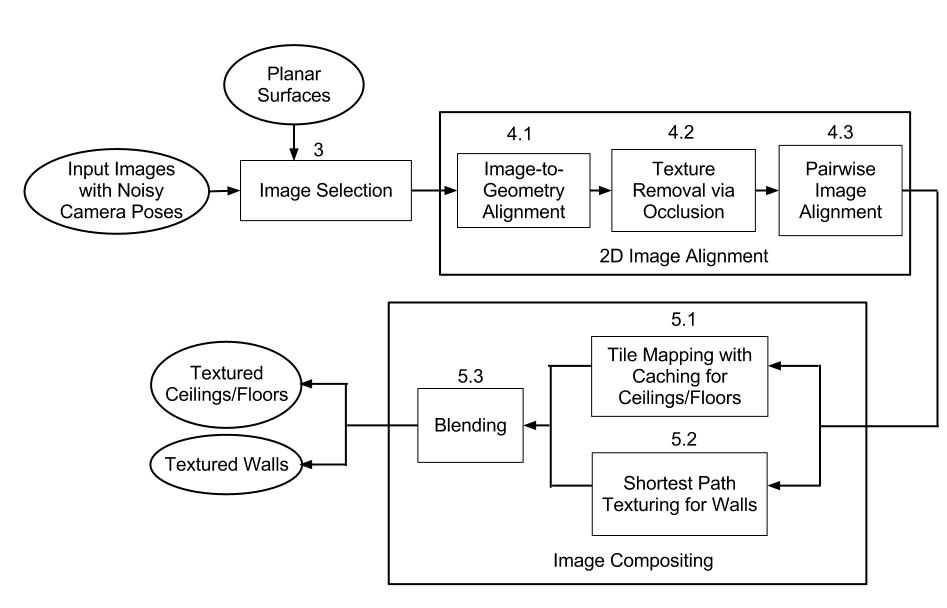
\includegraphics[width=6in]{flowchart.jpg}
  \caption{The proposed texture mapping procedure\\}
  \label{fig:flowchart}
\end{figure}


The overall block diagram for the proposed texture mapping procedure
is shown in Figure \ref{fig:flowchart}, where the number attached
attached to each box indicates the section in which the concept in the
box is explained in this paper. We texture map each planar surface
independently and in parallel. For each surface, we begin by selecting
a set of images that spans the entire surface with high resolution
imagery. We then use our noisy camera poses to project these selected
images onto the surface. These projections are then refined in 2D, in
order to maximally align them with the surface's geometry, as well as
to each other, allowing us to handle both errors in geometry as well
as camera poses. For surfaces and camera poses at arbitrary locations
or orientations, generally ceilings and floors, we propose a
tile-based approach for sampling high-resolution portions of images
and compositing them into a texture. In cases where cameras have
consistently perpendicular viewing angles to the surfaces under
consideration, generally walls, we demonstrate a superior approach
that leads to more seamless textures.

The remainder of the paper is organized as follows. Section
\ref{sec:existingApproaches} covers existing approaches to image
stitching, and their performance on our datasets. Section
\ref{sec:simpleTextureMapping} explains how to downsample the set of
available images by selecting those with the best orientation and
distance from surfaces under consideration. Section
\ref{sec:2dAlignment} contains our approach towards 2D image
alignment, followed by Section \ref{sec:imageCompositing}, which
describes two methods of selecting and compositing images to create
the final texture. Sections \ref{sec:results} and \ref{sec:conclusion}
contain results and conclusions.

%%%%%%%%%%%%%%%%%%%%%%%%%%%%%%%%%%%%%%%%%%%%%%%%%%%%%%%%%%%%%


\section{Existing Approaches to Image Alignment}
\label{sec:existingApproaches}
There are many existing approaches to stitching together multiple
images to produce a larger, seamless image \cite{szeliski2006image,
  agarwalapanoramas, wangmultipleviews, coorg1997matching,
  debevechybrid, bernardinimultiplescans}. Generally, parts of images
are matched to each other, either through direct comparisons or
feature detection and matching. Images are then transformed to
maximize matches, often by computing homographies between pairs of
images, or by iteratively adjusting camera poses in 1 to 6 degrees of
freedom.

Feature matching has a number of advantages over direct matching that
make it more suitable for our often non-planar environments, and
rotational differences between camera poses
\cite{szeliski2006image}. Feature matching however, works best when
multiple unique visual references exist in the environment that can be
detected in multiple images. In contrast, indoor environments have a
high prevalence of bare surfaces, as well as repeating textures, such
as similar windows, doors, and wall-mounted decorations, that are
difficult to disambiguate. This lack of reliable reference points
often results in errors when matching images together.

Additionally, our datasets often contain long chains of images,
corresponding to long hallways and corridors as shown in Figure
\ref{fig:mosaic3D}, which leads to error accumulation when image
correspondences are not accurate. For example, when matching a long
chain of images through homography, a pixel in the $nth$ image must be
translated into the first image's coordinates by multiplying by the
$3\times3$ matrix $H_1 H_2 H_3 ... H_n$. Any error in one of these
homography matrices is propagated to all further images, resulting in
drift.

\begin{figure}
  \centering \subfloat[][]{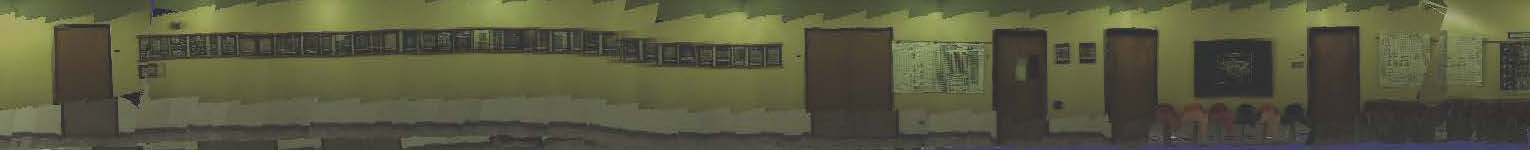
\includegraphics[trim=0cm 0cm 20cm 0cm,
    clip=true, width=6in, height=0.7in]{graphApproach.jpg}}

  \centering \subfloat[][]{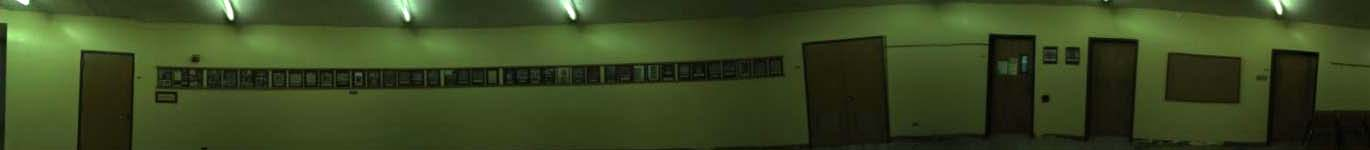
\includegraphics[trim=0cm 0cm 15cm 0cm,
    clip=true, width=6in, height=0.7in]{autostitchResult.jpg}}

  \centering \subfloat[][]{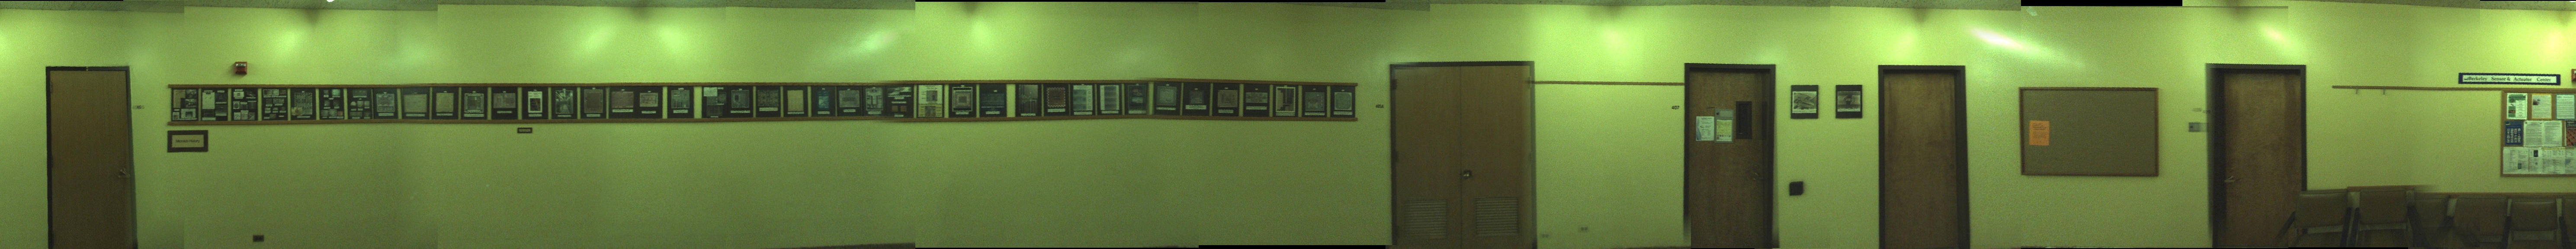
\includegraphics[trim=0cm 0cm 75cm 0cm,
    clip=true, width=6in, height=0.7in]{finalLong.jpg}}

  \caption{Texture alignment via (a) the graph-based localization
    refinement algorithm, (b) the AutoStitch software package, and (c)
    the proposed method.}
  \label{fig:mosaic3D}
\end{figure}


In prior work, we have experimented with integrating image stitching
with the iterative global localization algorithm used to recover the 6
degrees of freedom of the backpack acquisition system
\cite{liu2010indoor}. When run on long chains of images, especially
where features are sparse, this approach produces distorted textures,
as seen in Figure \ref{fig:mosaic3D}(a). Furthermore, this approach is
not closed-form, and its iterative camera adjustment process over
large datasets leads to prohibitively long computation time.

The AutoStitch software package performs homography-based alignment as
well, with additional provisions that attempt to reduce drift and
increase efficiency \cite{panorama2d, autostitch}. Though AutoStitch
performs well in areas with dense features, it can not handle areas
without features, and has trouble aligning wall sections with even
short segments of bare texture. The example in Figure
\ref{fig:mosaic3D}(b) has been generated after many rounds of manual
tuning; we have empirically found that areas with fewer visual
features or repeating texture patterns simply failed outright with
AutoStitch.

\section{Image Selection}
\label{sec:simpleTextureMapping}

The geometry of the texture mapping process for a planar surface is
shown in Figure \ref{fig:projection}. Given a set of $M$ images to
texture a target plane, camera matrix $P_i$ for the $ith$ image
transforms a 3D point in the world coordinate system to a 2D point or
pixel in image $i$'s coordinates. A camera matrix $P_i$ is composed of
the camera's intrinsic parameters, containing focal length and image
center, as well as extrinsic parameters which specify the rotation and
translation of the camera's position in 3D world coordinates at the
time that image $i$ is taken. These extrinsic parameters are
determined by the backpack hardware and the corresponding localization
algorithms \cite{chen2010indoor, liu2010indoor, kua2012loopclosure}
and are noisy.

Since the backpack system takes pictures at a rate of 5 Hz, hundreds
of images are available for texturing each surface in the 3D
model. Our objective in designing a texture mapping process is to
determine which of these images should be used, and where their
contents should map onto the final texture, in order to minimize any
visual discontinuities or seams that would suggest that the plane's
texture is not composed of a single continuous image. In the remainder
of this section, we propose an image selection criteria and use it to
derive a simple tile-based texture mapping procedure.

\begin{figure}
  \begin{minipage}[b]{0.45\linewidth}
    \centering
    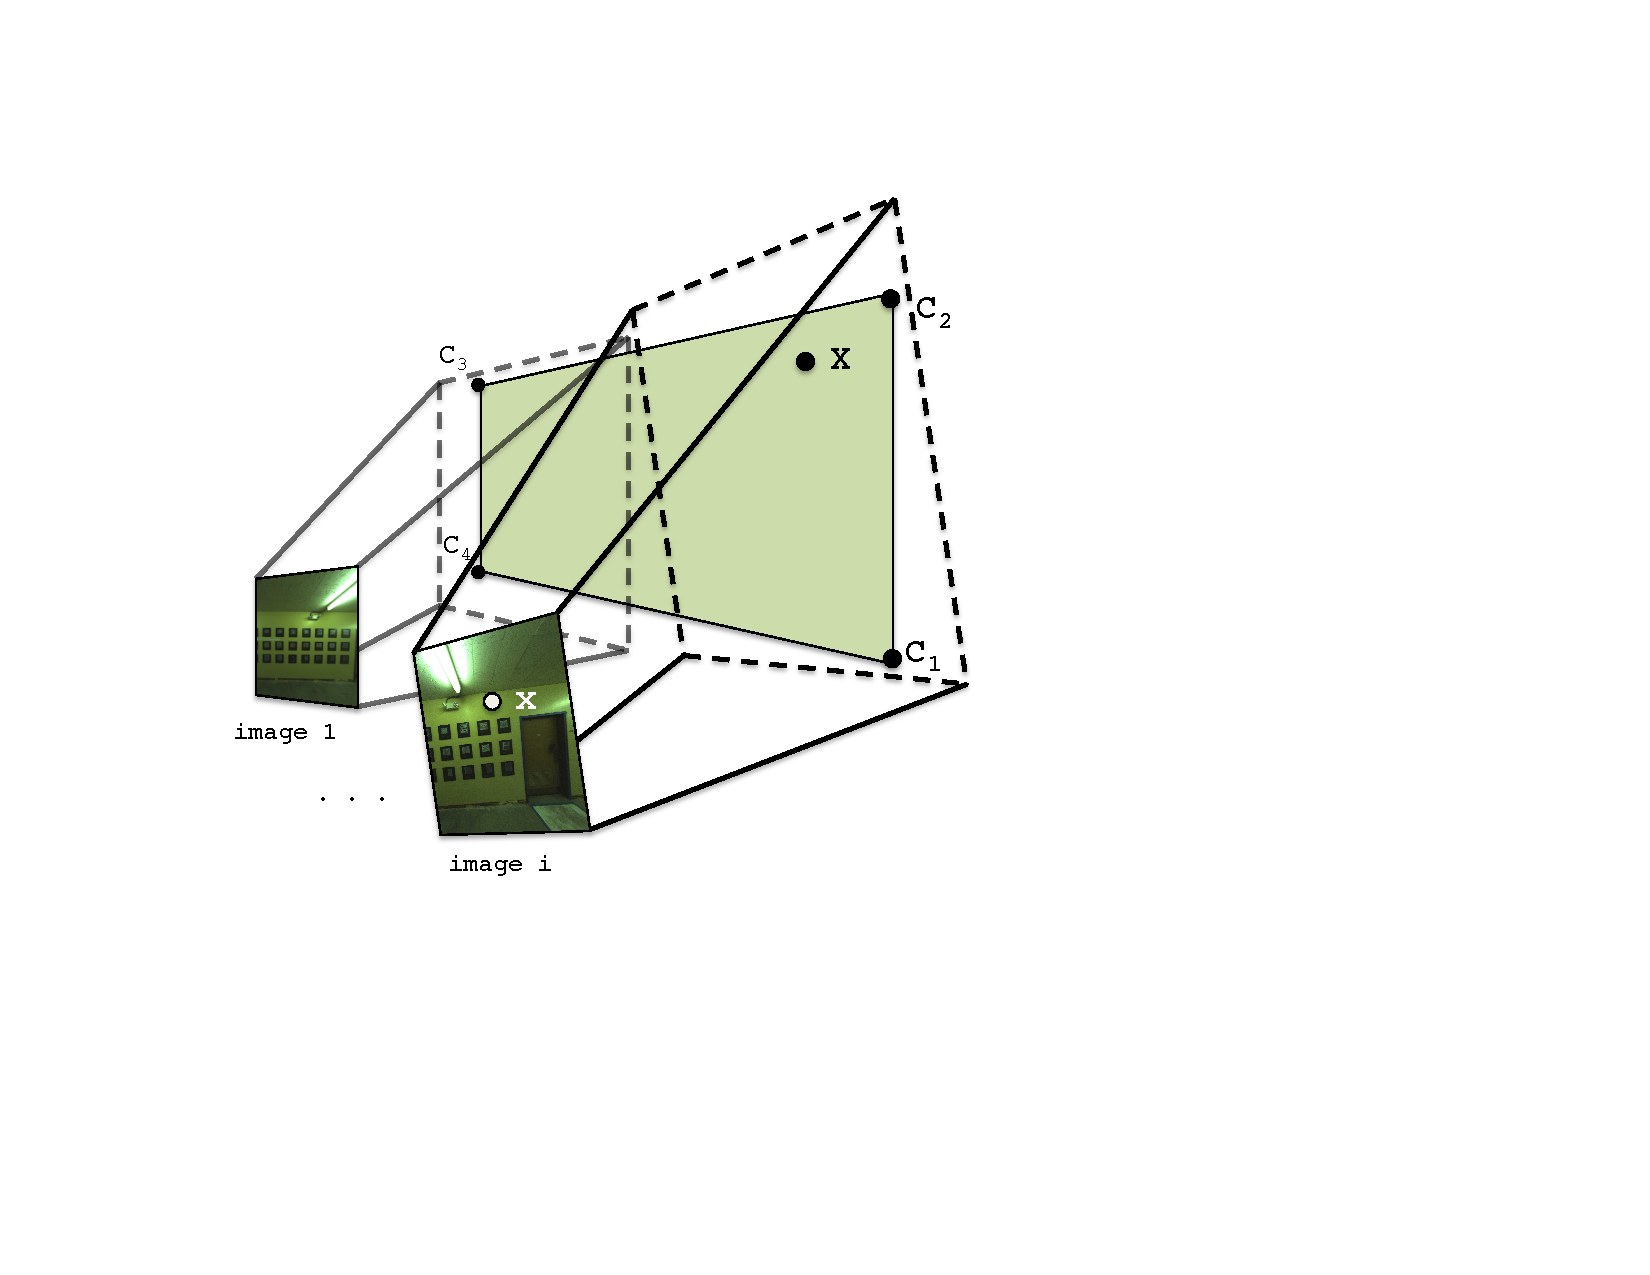
\includegraphics[height=1.8in]{Projection.pdf}
    \caption{Surfaces to be textured are specified in 3D space by
      corners $C_i$. Images are related to each surface through the
      camera matrices $P_{1..m}$. }
    \label{fig:projection}
  \end{minipage}
  \hspace{0.5cm}
  \begin{minipage}[b]{0.45\linewidth}
    \centering
    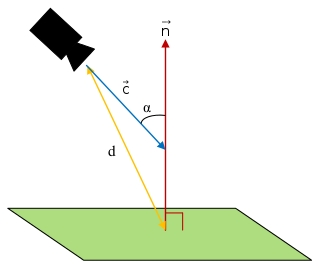
\includegraphics[height=1.8in]{scoringFunction.jpg}
    \caption{We minimize camera angle $\alpha$ and distance $d$ by
      maximizing the scoring function $\frac{1}{d} (-1 \cdot \vec{c})
      \cdot \vec{n}$}
    \label{fig:scoringFunction}
  \end{minipage}
\end{figure}


Ignoring the fact that the camera matrices $P_{1..M}$ are inaccurate,
a straightforward approach for texturing is to discretize the target
plane into small square tiles, and choose an image to texture each
tile directly. We choose to work with rectangular units to ensure that
borders between any two distinct images in the final texture are
either horizontal or vertical. Since most environmental features
inside buildings are horizontal or vertical, any visible seams in the
texture intersect them minimally and are therefore less noticeable.

In order to select an image for texturing a tile $t$, we first gather
a list of candidate images that contain all four of its corners; we
can rapidly check this by projecting $t$ into each image using the
$P_i$ camera matrices. Furthermore, each candidate image must have
been taken at a time when its camera had a clear line-of-sight to $t$,
which can be determined using standard ray-polygon intersection tests
between the camera location, $t$, and every other surface
\cite{rayintersection}.

Once we have a list of candidate images for $t$, we define a scoring
function in order to objectively select the best image for texturing
$t$. Since resolution decreases and camera pose errors become more
pronounced with distance, we wish to minimize the distance between
cameras and the surfaces they texture. Additionally, we desire images
that are projected perpendicularly, rather than obliquely, onto the
plane, maximizing the resolution and amount of useful texture
available in their projections, as well as minimizing any parallax
effects due to real-world geometry not accurately represented by the
digital 3D model. In other words, we wish to minimize the angle
between the tile's normal vector and the camera axis for images
selected for texturing that tile. These two criteria can be met by
maximizing the function $\frac{1}{d} (-1 \cdot \vec{c}) \cdot \vec{n}$
as shown in Figure \ref{fig:scoringFunction}, where $d$ is the
distance between the centers of a camera and a tile, and $\vec{n}$ and
$\vec{c}$ are the directions of the plane's normal and the camera axis
respectively. As Figure \ref{fig:compareAll}(a) demonstrates, this
approach, when used directly for texturing, results in image
boundaries with abrupt discontinuities between tiles, due to
misalignment between images, though most of it appears to be
reconcilable using 2D transforms.

While this procedure can be used to generate a texture, it is also
useful for obtaining a collection of images that can be used as a
starting point for our proposed texturing procedure, as explained in
Section \ref{sec:2dAlignment}. For our datasets, this process
generally selects around 10\% of all the images that could be used for
texturing the surface. This roughly 10:1 subsampling not only reduces
computational complexity of the remaining steps, but also selects the
most promising images for the remaining steps.

\begin{figure}
  \centering \subfloat[][]{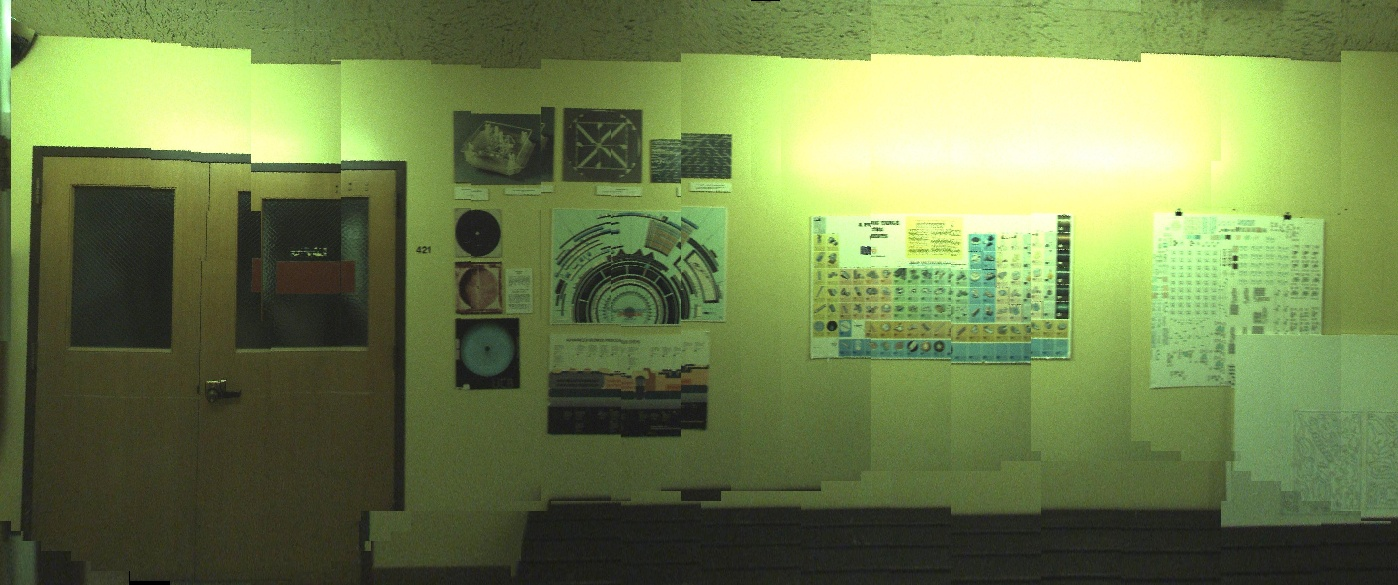
\includegraphics[width=3.4in,
    height=1.2in]{wall2_naive.jpg}}
  \subfloat[][]{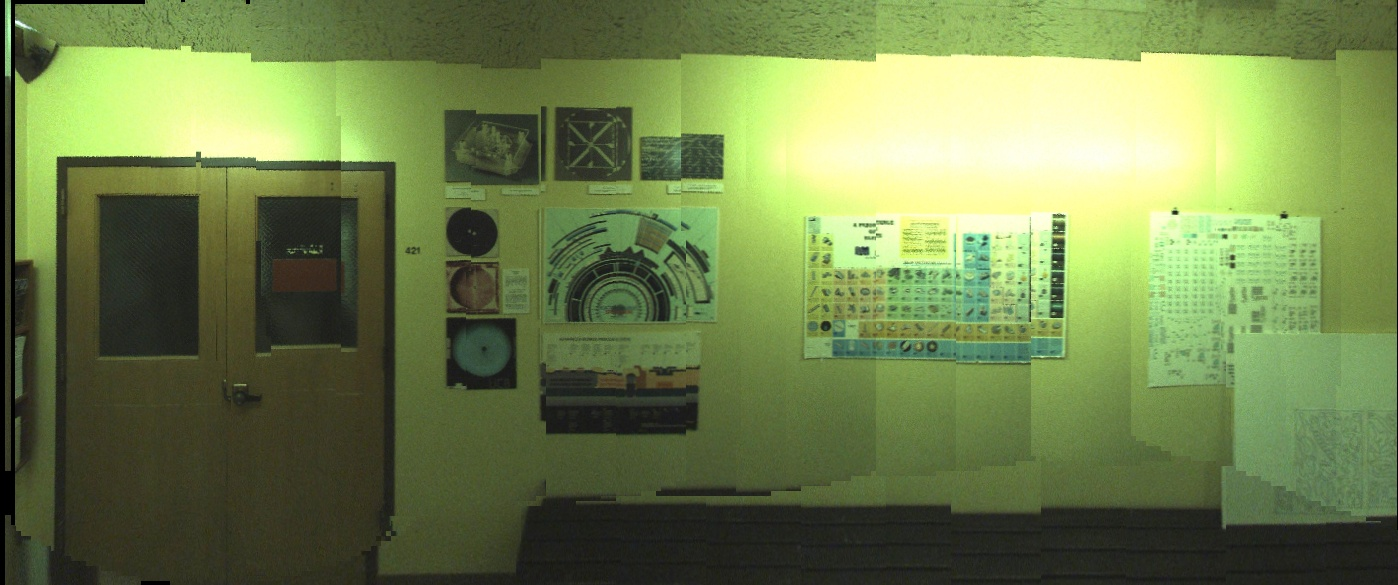
\includegraphics[width=3.4in,
    height=1.2in]{wall2_naive_shift.jpg}}

  \centering \subfloat[][]{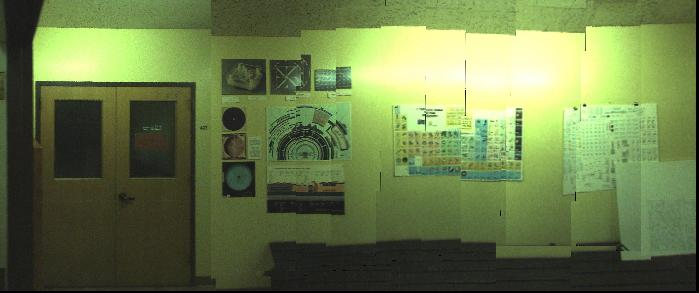
\includegraphics[width=3.4in,
    height=1.2in]{wall2_cache_shift.jpg}}
  \subfloat[][]{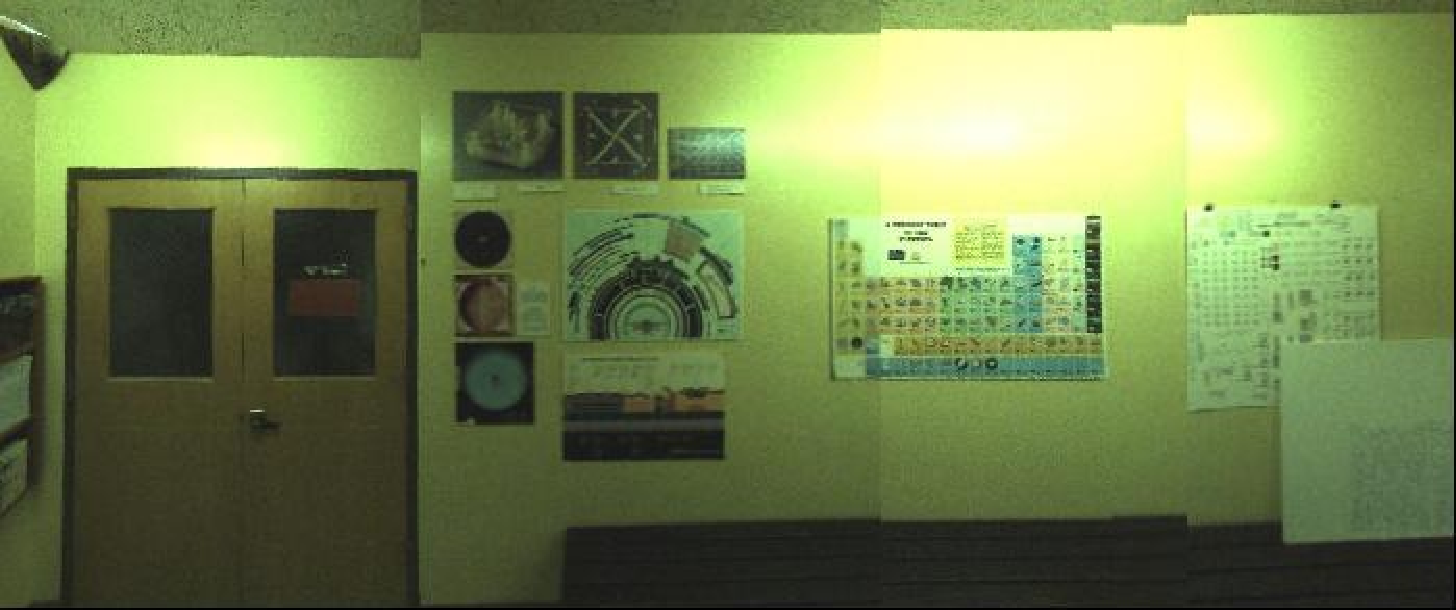
\includegraphics[width=3.4in,
    height=1.2in]{wall2_shortest_shift.pdf}}

  \centering \subfloat[][]{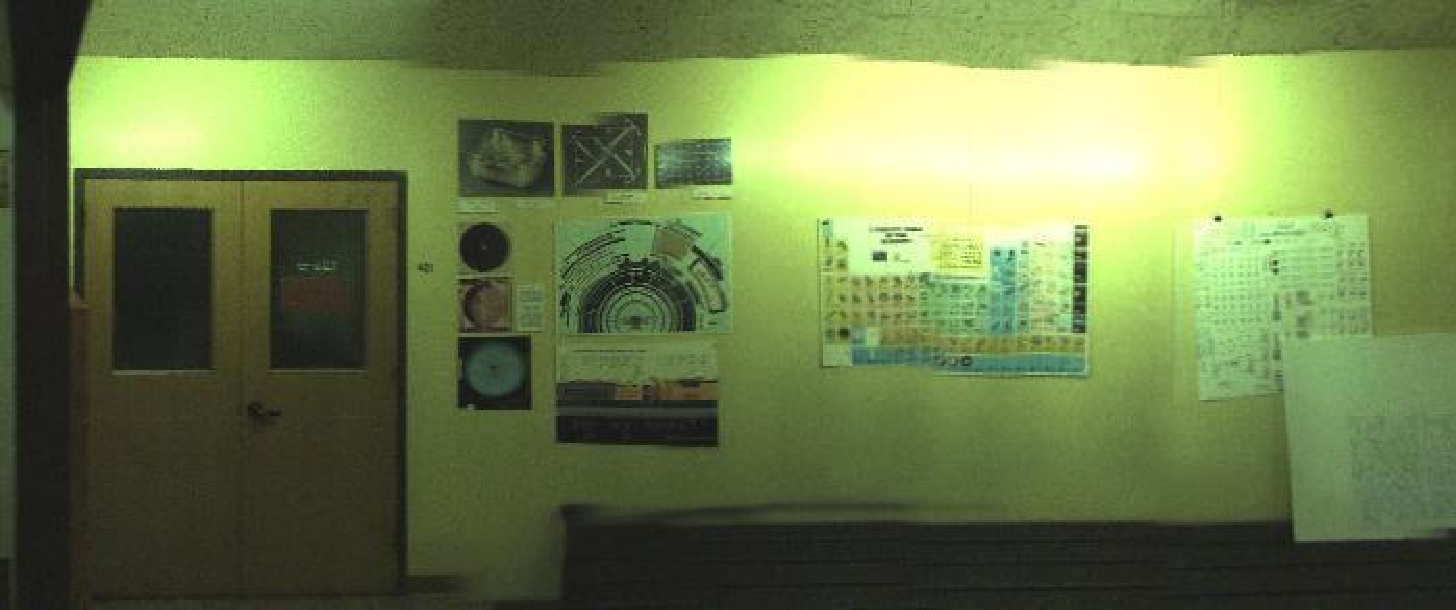
\includegraphics[width=3.4in,
    height=1.2in]{wall2_cache_shift_blend.pdf}}
  \subfloat[][]{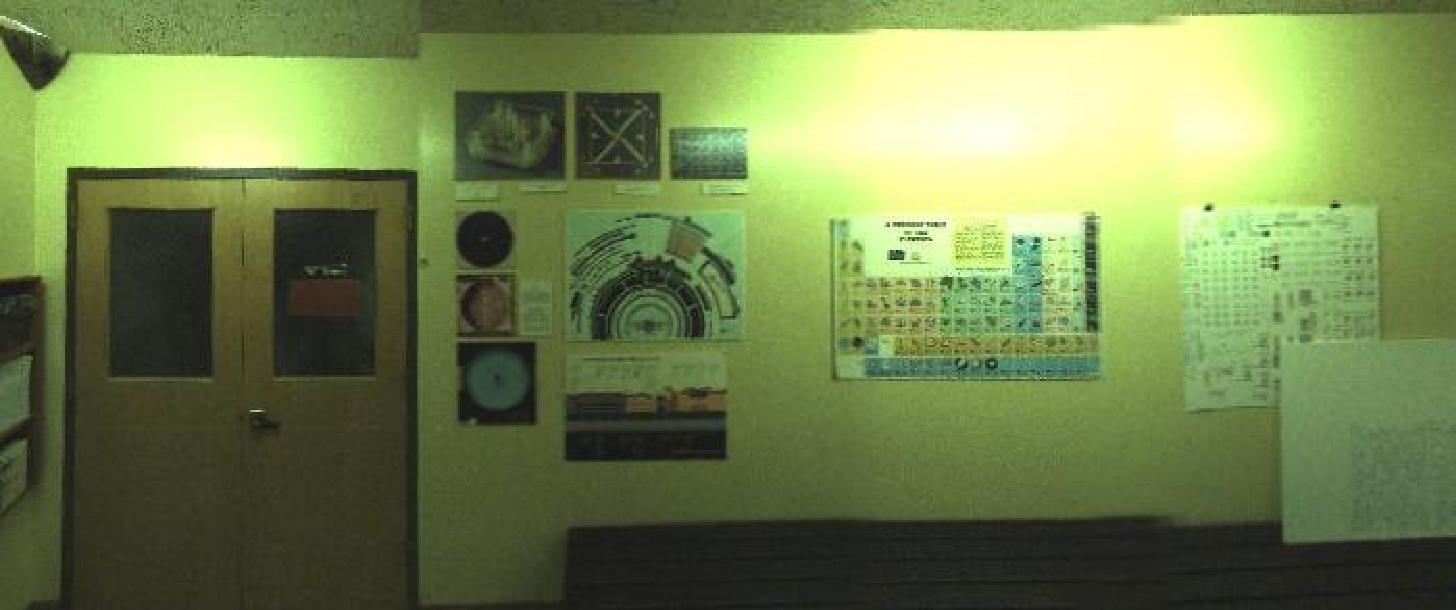
\includegraphics[width=3.4in,
    height=1.2in]{wall2_shortest_shift_blend.pdf}}

  \centering \subfloat[][]{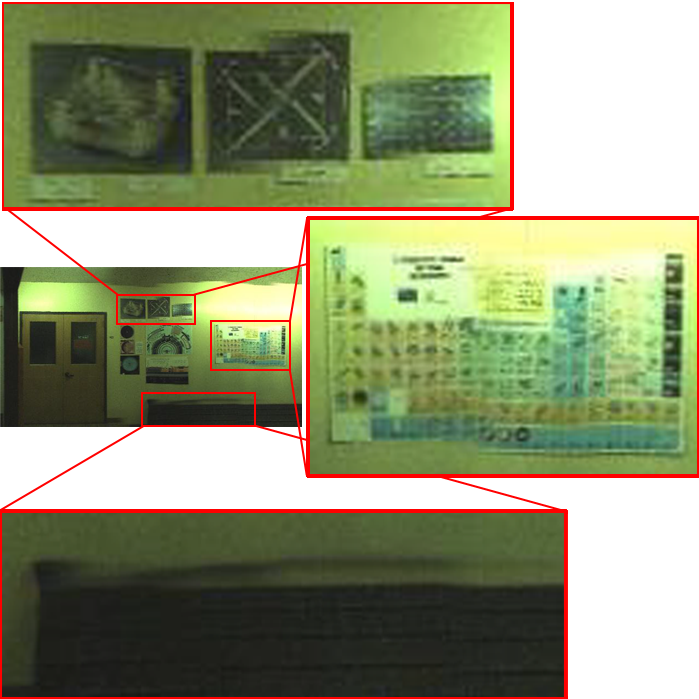
\includegraphics[width=3.4in,
    height=3.4in]{wall2_cache_comparison.png}}
  \subfloat[][]{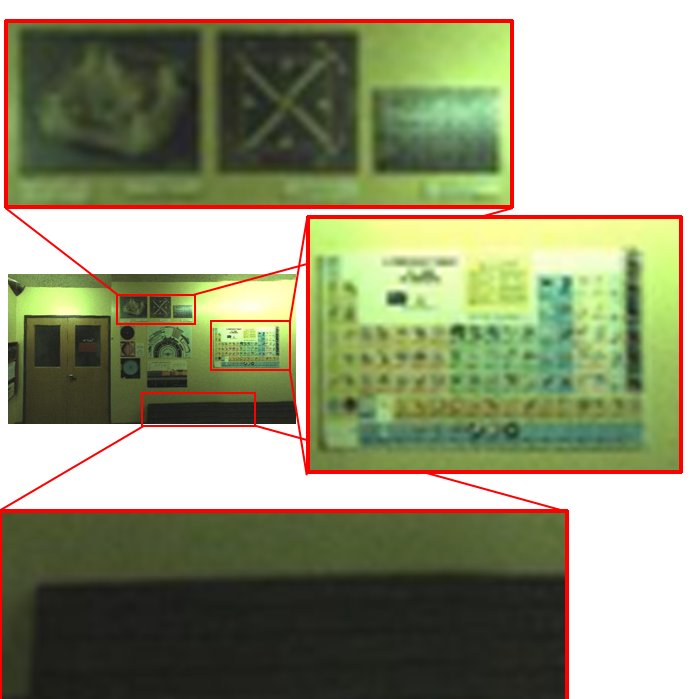
\includegraphics[width=3.4in,
    height=3.4in]{wall2_shortest_comparison.png}}

  \caption{(a) Tile-based texturing; (b) Tile-based texturing after
    image alignment; (c) Tile-based texturing after image alignment
    with caching; (d) Shortest path texturing after image
    alignment; (e,f) Blending applied to (c) and (d); (g,h) Zoomed
    in views of discontinuities in (e) vs. in (f).}
  \label{fig:compareAll}
\end{figure}


\section{2D Image Alignment}
\label{sec:2dAlignment}
In this section, we describe our method for efficient and robust image
alignment. Rather than register all of our images in 3D, as many
state-of-the-art techniques for image stitching do, we instead select
a subset of images to be aligned in 2D. This subset corresponds to the
images selected by the image selection procedure described in Section
\ref{sec:simpleTextureMapping}.

Applying 2D alignments to this set of images works well for a number
of reasons. First, the nature of our input data and the selected
images is such that localization error chiefly occurs in two
dimensions, which correspond to the plane of the surface being
projected onto. This is because the backpack operator, during data
acquisition, makes efforts to walk within a few meters of, and
parallel to all walls being scanned. As a result, the translational
error of camera poses is quite minimal in the dimension perpendicular
to the wall surface being textured. Furthermore, because our set of
images has minimal distance from its corresponding wall surface,
rotational errors are less pronounced, except for rotation around the
axis perpendicular to the surface being textured. Therefore, most
translation and rotational errors occur in the 2 dimensions of the
wall surface's plane. This of course does not apply for ceilings and
floors; however, the lack of features on most ceilings and floors
means that 3D misalignment is not likely to visually make a
difference, beyond what can be done in 2D.


Our proposed 2D alignment procedure consists of three parts, as shown
in the diagram in Figure \ref{fig:flowchart}. First, images are
projected onto the surface and lines within these projected images are
detected. Images are then transformed such that these lines match
geometric lines composing the boundaries of the surface being
textured. Second, occlusion checks are performed to remove invalid
parts of each image for the target surface. Third, SIFT feature
matches are detected between pairs of images, and a weighted linear
least squares problem is solved in order to maximize all image and
geometry-based alignments. Each step will now be explained in detail.


\subsection{Geometry-based Alignment}
\label{sec:geometryAlignment}


\begin{figure}
  \centering
  \subfloat[][]{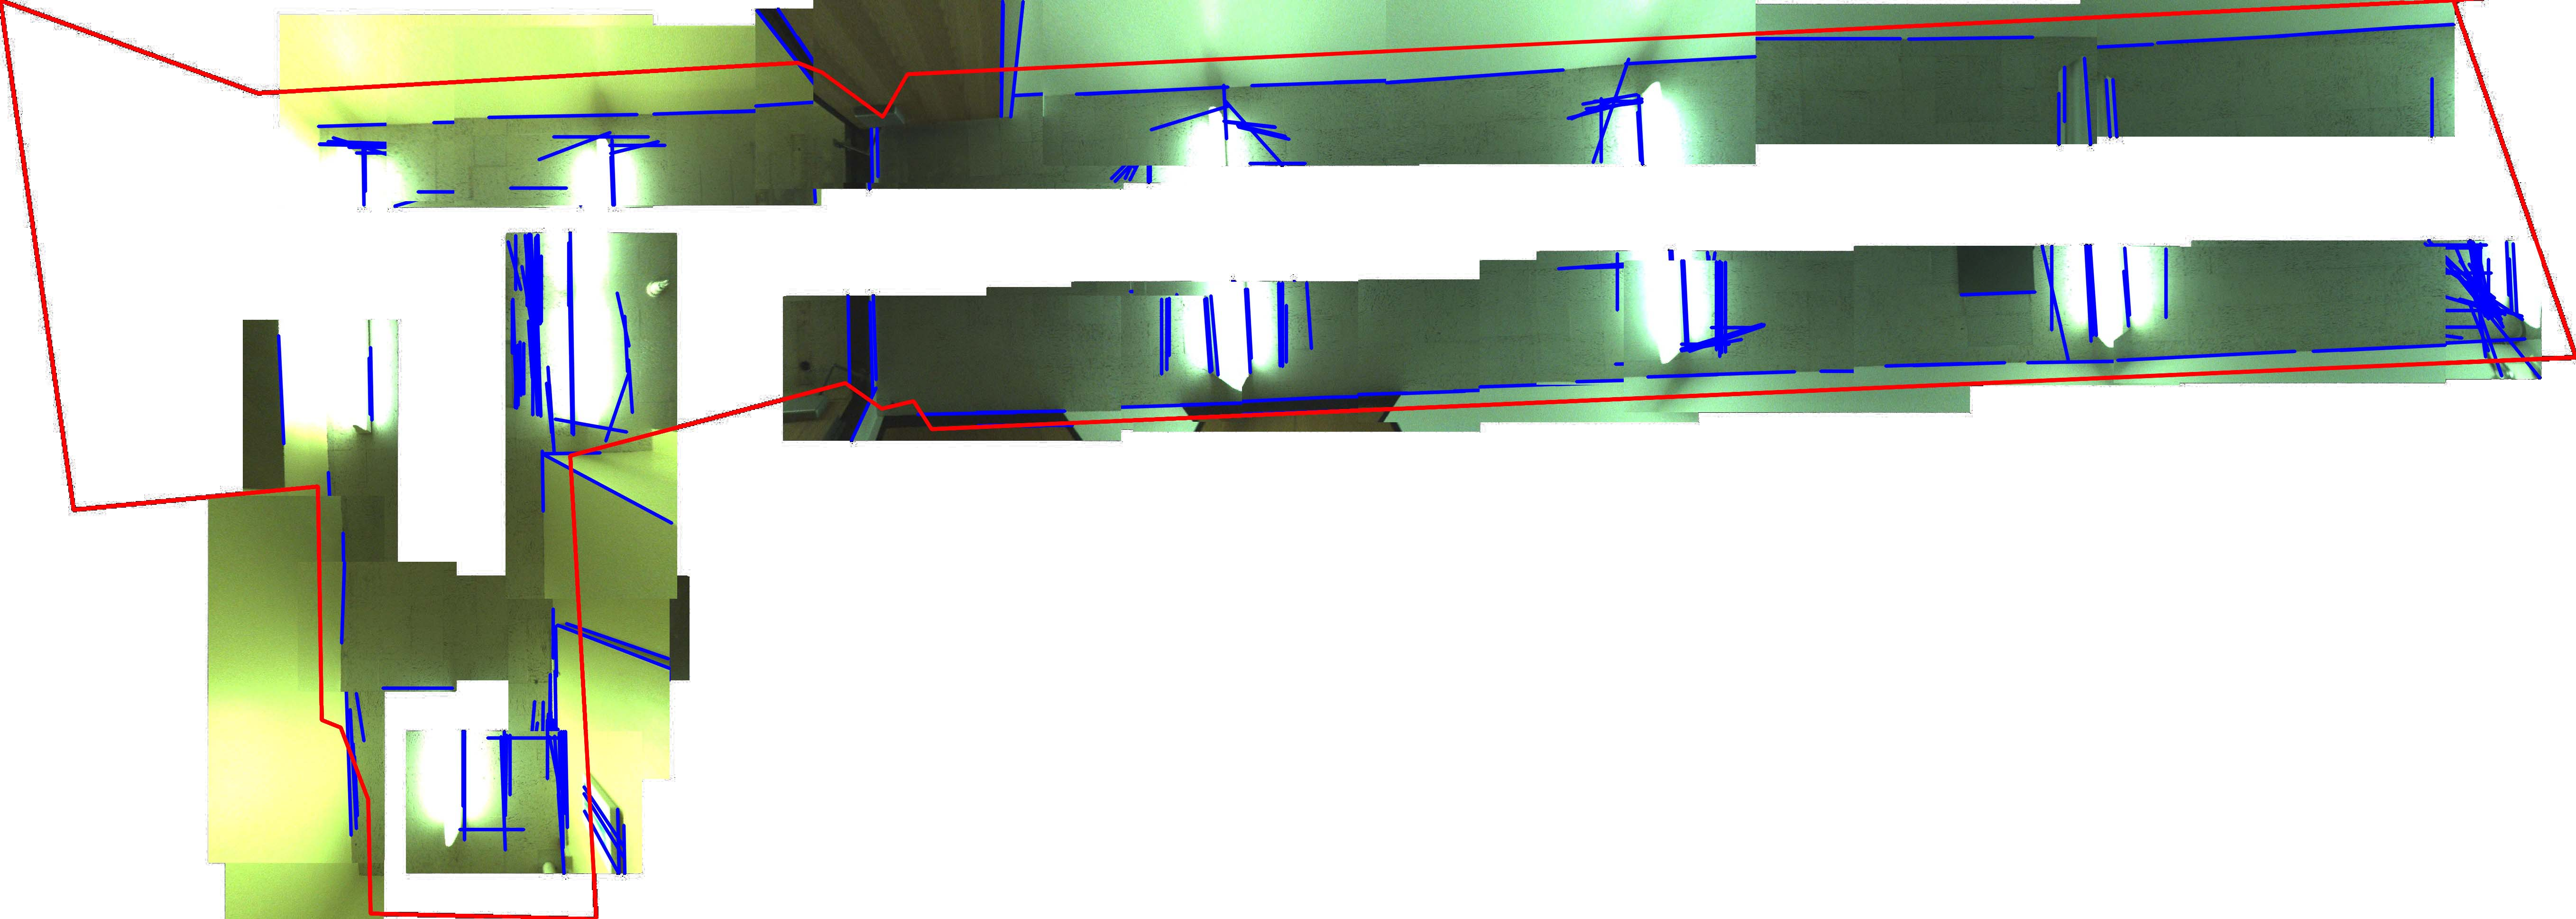
\includegraphics[width=6in]{allunshifted.jpg}}

  \centering
  \subfloat[][]{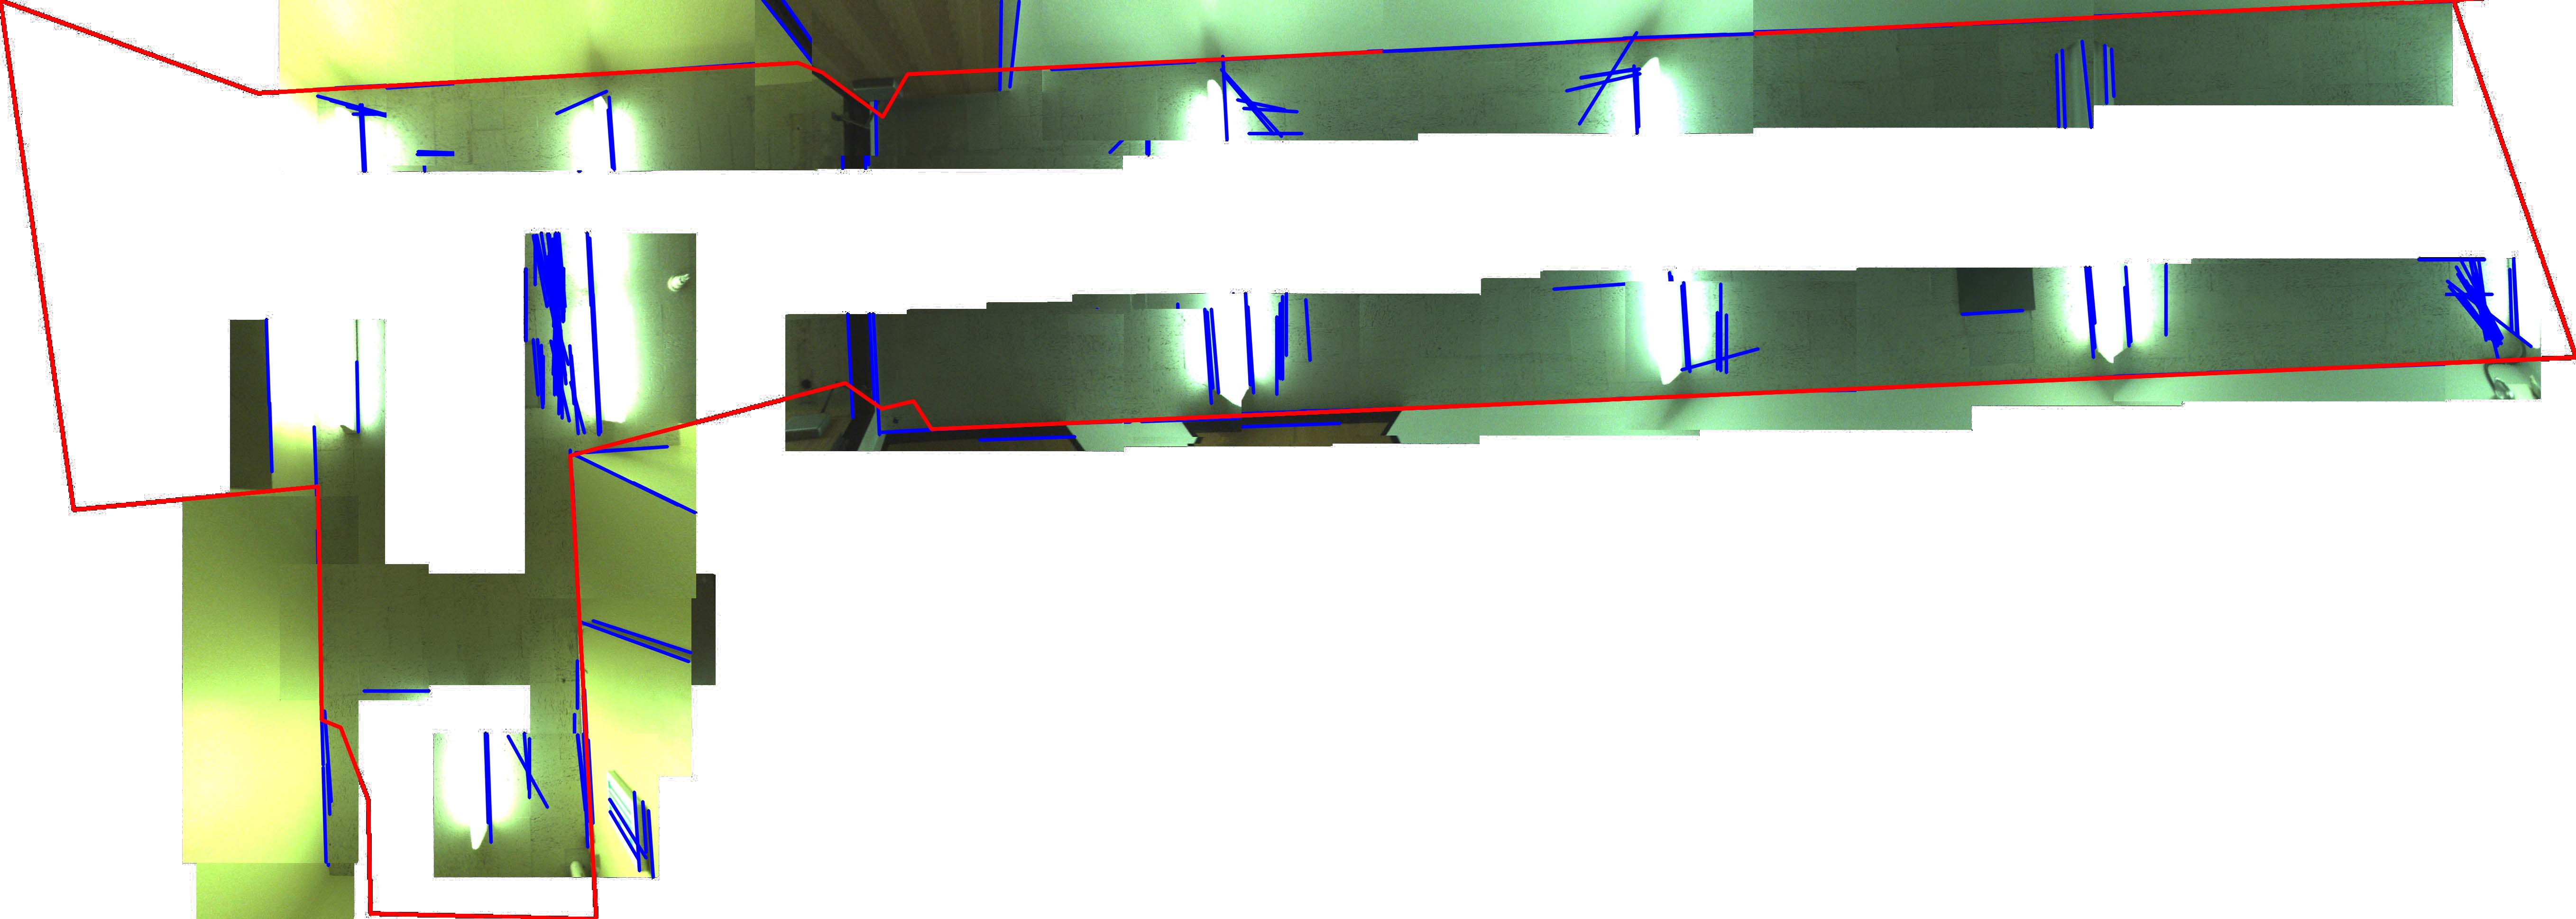
\includegraphics[width=6in]{allshifted.jpg}}

  \centering \subfloat[][]{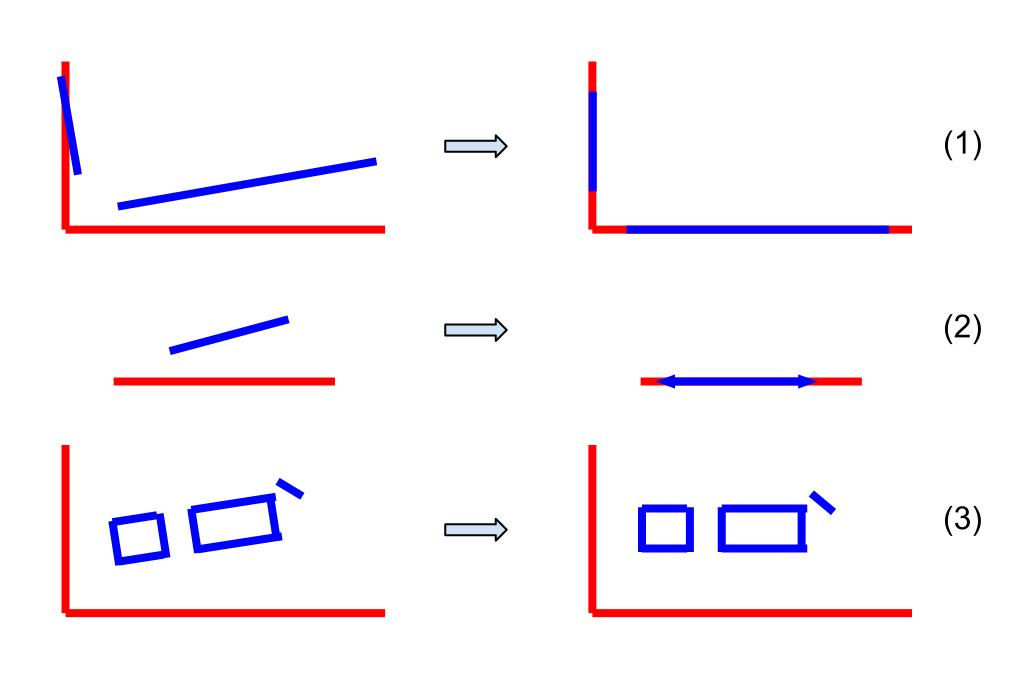
\includegraphics[trim=0cm 2cm 0cm 0cm,
    clip=true, width=5in]{matchLines.jpg}}

  \caption{Images projected onto a ceiling surface, where
    geometry-based lines corresponding to the ceiling's boundary are
    shown in red. Image-based lines detected by Hough transform in the
    image projections are shown in blue; (a) images projected with
    their original noisy camera poses; (b) after image alignment to
    maximize line matches between images and geometry; (c) examples of
    matching lines in cases with $\geq$ 2 line pairs, 1 line pair, and
    zero line pairs, from top to bottom.}
  \label{fig:geometryAlignment}
\end{figure}


After computing each image's projection onto the target surface, as
described in Section \ref{sec:simpleTextureMapping}, we obtain a set
of image-based line segments by using Hough transforms to detect lines
in the image projections. These lines are detected in the image
projections rather than the original images, as the varying
orientation and distances of camera poses relative to surfaces results
in high variance of line lengths and strengths for real-world linear
features across the original images. We also gather a set of
geometry-based lines, which correspond to the lines comprising the
target surface's border, as well as lines formed where other surfaces
intersect the target surface. An example of these lines is shown in
red for a ceiling surface in Figure
\ref{fig:geometryAlignment}(a). Ideally, for perfect camera poses and
surface geometry, the lines in images corresponding to corners between
surfaces should match up exactly with corners in the 3D model. By
inducing such lines to match, we fit camera poses more accurately to
the surface, and to each other as well.

To align images to surface geometry, we collect pairs of image-based
and geometry-based line segments, which are within a distance and
angular difference threshold of each other. We have found a distance
threshold of 250 mm and an orientation difference threshold of
$10^\circ$ to work well for our datasets. For each pair of lines, we
compute the angular difference between the pair's image and geometry
lines. If there are 2 or more pairs with angular differences within
$1^\circ$, we select the two pairs with the longest noncollinear
image-based lines, and rotate the image such that the lines in the
pair with the longest image-based line become parallel. We then find a
translation such that the lines in that same pair overlap. This
translation has ambiguity in the dimension along the matched lines,
which is resolved by matching the midpoint of the image-based line in
the second pair to its corresponding geometry-based line. This is
shown in case (1) of Figure \ref{fig:geometryAlignment}(c). Thus, with
2 or more pairs, it is possible to obtain a fixed rotation and
translation, which are saved for usage in Section
\ref{sec:robustSIFTFeatureMatching}.

If there are not 2 or more pairs with similar angular differences, we
select the pair with the longest image-based line and apply a rotation
and the minimal translation to match its lines. This translation's
ambiguity however, can not be resolved, but is also saved to be used
in Section \ref{sec:robustSIFTFeatureMatching}. This is shown in case
(2) of Figure \ref{fig:geometryAlignment}(c). Finally, in the case
where there are no line pairs, we can still rotate images in order to
exploit patterns in indoor environments, as shown in case (3) of
Figure \ref{fig:geometryAlignment}(c). For instance, doors, windows,
furniture, etc. tend to have linear edges that are parallel to the
edges of the surfaces they are on. Similarly, lights, visible interior
walls, etc. which are visible in floor and ceiling images, tend to be
parallel to exterior walls corresponding to the edges of ceiling and
floor surfaces. Thus, we choose to minimize the angle between
image-based lines and geometry-based lines. We use the RANSAC
framework, with an inlier difference of $0.5^\circ$ in order to
successfully ignore outliers \cite{fischler1981random}.

After these steps, image projections line up well with target
surfaces, as shown in Figure \ref{fig:geometryAlignment}(b), which is
considerably more aligned than Figure
\ref{fig:geometryAlignment}(a). This procedure reconciles both errors
in camera poses as well as in geometry, and results in sharp,
continuous borders across images, which is crucial when checking for
occlusion.


\subsection{Image Occlusion}
\label{sec:imageOcclusion}

\begin{figure}
  \centering
  \begin{tabular}{cc}
    \subfloat[][]{\raisebox{-1in}{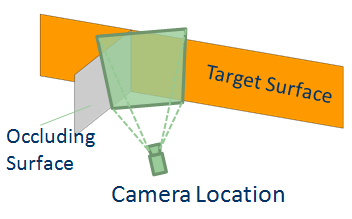
\includegraphics[width=3in]{occlusiondiagram.png}}} &
 
  \begin{tabular}{c}
    \subfloat[][]{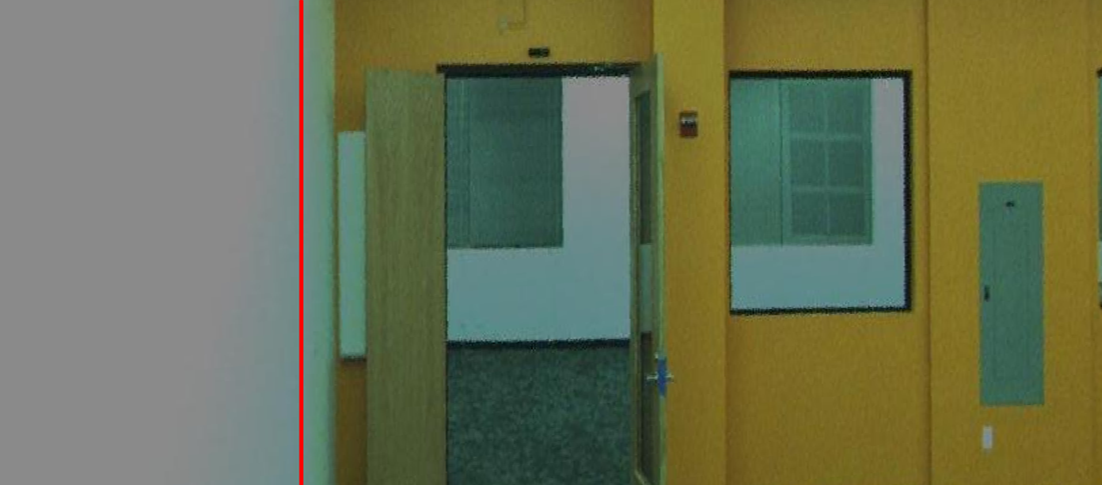
\includegraphics[trim=0cm 0cm 1.3cm 0cm,
      clip=true, width=3in,
      height=0.9in]{occlusionimagebad.png}} \\
    \subfloat[][]{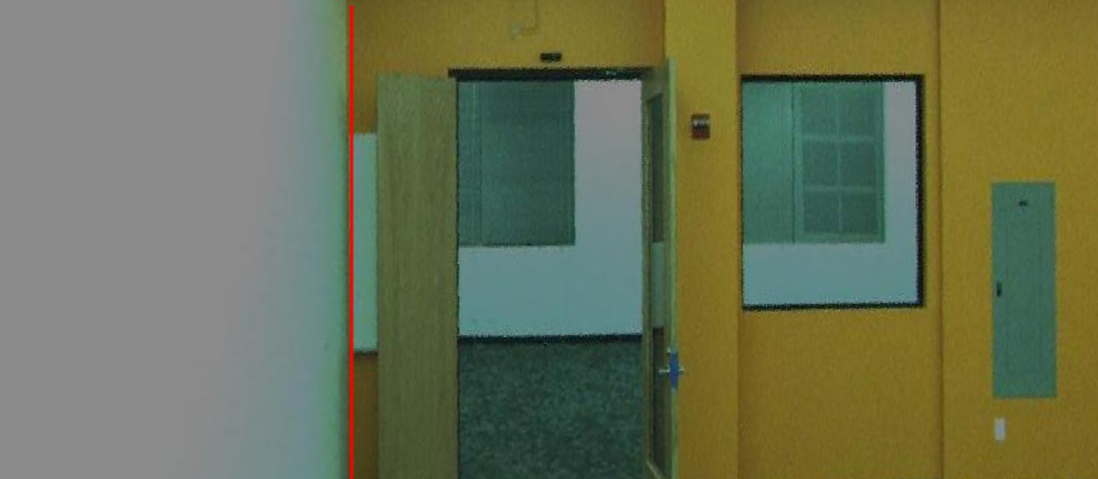
\includegraphics[trim=1.3cm 0cm 0cm 0cm,
      clip=true, width=3in,
      height=0.9in]{occlusionimagegood.png}}
  \end{tabular}
\end{tabular}
\caption{(a) The image from the camera in this diagram contains
  texture that belongs to the gray occluding surface, which should not
  be projected onto the orange target surface; (b) without geometry
  alignment, texture to the left of the red line would be removed,
  which would leave some erroneous texture projected onto our target
  surface; (c) after geometry alignment, the image is shifted,
  resulting in the correct amount of texture being removed.}
\label{fig:occlusion}
\end{figure}

In order to correctly texture surfaces, it is important to detect and
remove parts of image projections containing texture for occluding
surfaces. For instance, in Figure \ref{fig:occlusion}(a), an image
used to texture the orange target surface also contains part of a gray
occluding surface. We remove this incorrect texture by recursively
performing ray-polygon intersection tests between the camera location
and every surface in our model except the target surface
\cite{rayintersection}. These intersection tests are performed at the
corners of a grid overlaid upon the target surface. Where all four
corners of a grid section are occluded, texture is removed. Where one
or more corners are occluded, the grid is subdivided into four, and
the process repeats. Occlusion checking works entirely with geometry,
so by ensuring that images match geometry using
\ref{sec:geometryAlignment}'s alignment procedure, texture belonging
to other surfaces is accurately removed, as seen in Figure
\ref{fig:occlusion}(b).

\subsection{2D Feature Alignment}
\label{sec:robustSIFTFeatureMatching}
The next step is to align the selected images from Section
\ref{sec:simpleTextureMapping} for each surface to each other by
searching for corresponding feature points between all pairs of
overlapping images. We use feature alignment rather than pixel or
intensity-based alignment due to the differences in lighting as well
as possible occlusion among images, both of which feature alignment is
less sensitive to \cite{lowe1999object, mikolajczyk2005performance,
  szeliski2006image}. We use SiftGPU \cite{siftgpu} for its high
performance on both feature detection as well as pairwise
matching. These matches determine $dx$ and $dy$ distances between each
pair of features for two image projections, though these distances may
not always be the same for different features. Since indoor
environments often contain repetitive features such as floor tiles or
doors, we need to ensure that SIFT-based distances are
reliable. First, we only align parts of images that overlap given the
original noisy poses. Second, we discard feature matches that
correspond to an image distance greater than 200 mm from what the
noisy poses estimate. In order to utilize the remaining feature
matches robustly, RANSAC \cite{fischler1981random} is again used to
estimate the optimal $dx_{i,j}$ and $dy_{i,j}$ distances between two
images $i$ and $j$. We use a 5 mm threshold for RANSAC, so that SIFT
matches are labeled as outliers if their distance is not within 5 mm
of the sampled average distance.


We now use the feature-based distances between each pair of images as
well as geometry alignment results from Section
\ref{sec:geometryAlignment} to refine all image positions using a
weighted linear least squares approach. An example setup for a
weighted linear least squares problem $\textrm{min}_{\vec{\beta}}
||W^\frac{1}{2}(A \vec{\beta} - \vec{\gamma})||_2^2 $ with 3 images is
as follows.

\[
A =
\begin{pmatrix}
  -1 & 1 & 0 & 0 & 0 & 0\\
  0 & 0 & 0 & -1 & 1 & 0\\
  0 & -1 & 1 & 0 & 0 & 0\\
  0 & 0 & 0 & 0 & -1 & 1\\
  0 & -m_2 & 0 & 0 & 1 & 0\\
  1 & 0 & 0 & 0 & 0 & 0\\
  0 & 0 & 0 & 1 & 0 & 0\\
  1 & 0 & 0 & 0 & 0 & 0\\
  0 & 0 & 0 & 1 & 0 & 0\\
  0 & 1 & 0 & 0 & 0 & 0\\
  0 & 0 & 0 & 0 & 1 & 0\\
  0 & 0 & 1 & 0 & 0 & 0\\
  0 & 0 & 0 & 0 & 0 & 1\\


\end{pmatrix}\quad
\vec{\beta} =
\begin{pmatrix}
  x_1, \\ x_2, \\ x_3, \\ y_1, \\ y_2, \\ y_3
\end{pmatrix}
\vec{\gamma} =
\begin{pmatrix}
  dx_{1,2}, \\ dy_{1,2}, \\ dx_{2,3}, \\ dy_{2,3}, \\ -m_2gx_2 + gy_2,
  \\ gx_1, \\ gy_1, \\ tx_1, \\ ty_1, \\ tx_2, \\ ty_2, \\ tx_3, \\
  ty_3
  
\end{pmatrix}
\vec{W} =
\begin{pmatrix}
  1, \\ 1, \\ 1, \\ 1, \\ 1, \\ 1, \\ 1, \\ 0.01, \\ 0.01, \\ 0.01, \\
  0.01, \\ 0.01, \\ 0.01
\end{pmatrix}
\]


The variables we wish to solve for are the $x_i$ and $y_i$ positions
of images, while equations are the feature-based distances between
pairs of images, images fixed to geometry with 0 or 1 degrees of
freedom, and the original noisy camera poses. In this scenario, a
feature-based distance of $dx_{1,2}$, $dy_{1,2}$ was calculated
between images 1 and 2. This corresponds to the first and second row
of $A$, while the third and fourth row of $A$ represent the same for
images 2 and 3. Rows 5 through 7 correspond to results of the geometry
alignment procedure in Section
\ref{sec:geometryAlignment}. Specifically, row 5 corresponds to a
geometry-based constraint of image 2's location to a line of slope
$m_2$, passing through point $gx_2$, $gy_2$, while rows 6 and 7
correspond to a fixed location for image 1 without any degrees of
freedom. Rows 8 through 13 correspond to the original camera locations
for each image ($tx_i,ty_i$).

The original camera poses are needed due to lack of feature matches in
all images, or lack of enough geometry alignment results to generate a
single solution. Since it is desirable to minimally use the original
noisy poses, we assign to them a weighting factor of $0.01$, while all
other equations are weighted at $1$.


Since this problem is linear, it can be solved efficiently; after
applying the resulting shifts, images overlap and match each other
with far greater accuracy. Using the simple tile-based texturing
scheme from Section \ref{sec:simpleTextureMapping} on these adjusted
images results in Figure \ref{fig:compareAll}(b), which has far fewer
discontinuities than in \ref{fig:compareAll}(a), though some 3D error
as well as lighting differences and parallax effects are still
visible.

\section{Image Compositing}
\label{sec:imageCompositing}
In Section \ref{sec:simpleTextureMapping} we described an image
selection method that reduces the list of candidate images for
texturing by a factor of 10. In this section we go one step further to
choose a subset of the above candidates in order to further reduce
visual artifacts and discontinuities across textured
surfaces. Specifically, in Section \ref{sec:mappingWithCaching}, we
refine the tile-based texturing approach from Section
\ref{sec:simpleTextureMapping}, with an added caching mechanism to
reduce image boundaries. This method is general and works well given
arbitrary camera poses and surfaces such as walls, floors, and
ceilings. For special cases where images have consistently
perpendicular viewing angles to the surfaces under consideration, such
as walls, it is possible to develop an alternative method in Section
\ref{sec:shortestPath} to further reduce visual artifacts. Both of
these approaches are followed by a blending step in order to produce
final textures for each surface, as shown in Figure
\ref{fig:flowchart}.

\subsection{Tile-Mapping with Caching}
\label{sec:mappingWithCaching}
For the simple texture mapping method described in Section
\ref{sec:simpleTextureMapping}, discontinuities occur where adjacent
tiles are textured by different images. Though Section
\ref{sec:2dAlignment}'s image alignment removes many such
discontinuities, there are still cases where seams are visible due to
imprecise matching or other factors such as model-based errors as
shown in Figure \ref{fig:compareAll}(b). To reduce this, it is
desirable to develop a spatiotemporal caching mechanism to take into
account image selections made by neighboring tiles while texture
mapping a given tile. By using the same image across tile boundaries,
it is possible to eliminate a discontinuity altogether. If a tile is
not visible in images used by neighboring tiles, using similar images
across tile boundaries also leads to less noticeable discontinuities.

The best image for a tile $t$ is selected by searching through two
subsets of images for a viable candidate, before searching through the
entire set of valid images obtained in Section
\ref{sec:simpleTextureMapping}. The first subset of images is those
selected by adjacent tiles that have already been textured. We must
first check which of these images contain texture for $t$, and then of
those, we make a choice according to the scoring function in Figure
\ref{fig:scoringFunction}. Before reusing this image, we check the
criteria $\alpha < 45^\circ$, in order to ensure a high resolution
projection, with $\alpha$ as the camera angle as shown in Figure
\ref{fig:scoringFunction}.

If no satisfactory image is found in the first subset, we check a
second subset of images, consisting of those taken near the ones in
the first subset, both spatially and temporally. We use the noisy
camera poses to determine spatial proximity. These images are not the
same as the ones used for neighboring tiles, but are taken at a
similar location and time, suggesting that their localization and
projection are quite similar, and thus likely match more
seamlessly. If no viable image is found according to the $\alpha <
45^\circ$ criteria, we search the entire set of candidate images from
Section \ref{sec:simpleTextureMapping}, selecting based on the same
scoring function from Figure \ref{fig:scoringFunction}.

The result of applying this caching approach to the images for the
surface in Figure \ref{fig:compareAll}(a) is shown in Figure
\ref{fig:compareAll}(c), where seams are considerably reduced as
compared to Figure \ref{fig:compareAll}(b). However, some
discontinuities are still present, as visible in the posters on the
wall with breaks in their borders.

\begin{figure}
  \centering
  \subfloat[][]{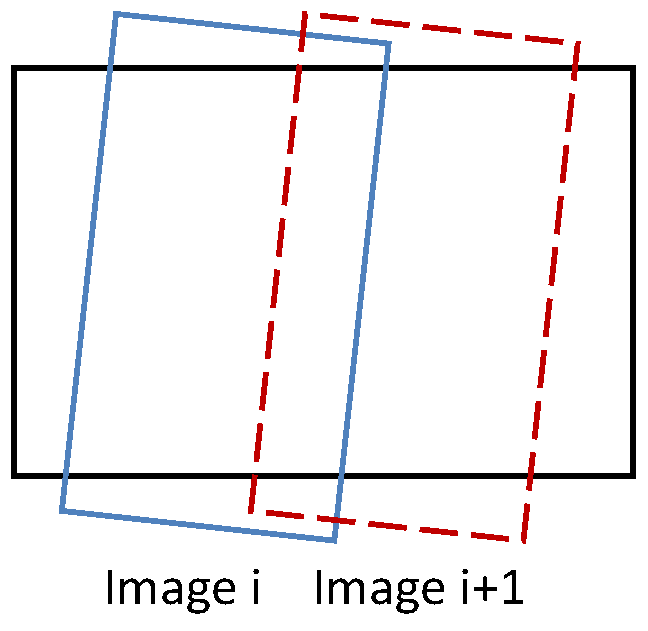
\includegraphics[width=1in]{projectionWall.pdf}}
  \hspace{1in} \centering
  \subfloat[][]{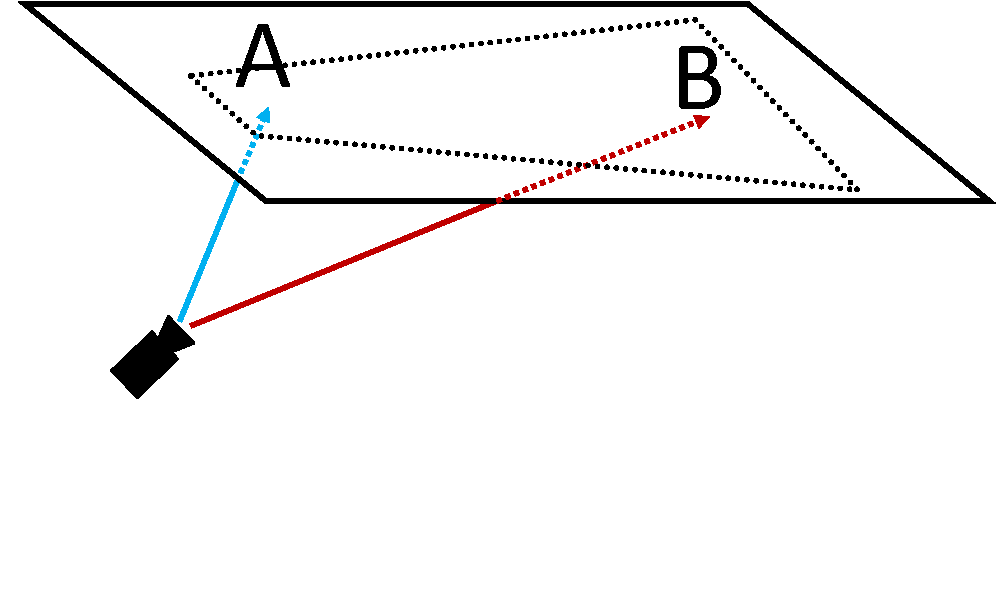
\includegraphics[width=1.1in]{projectionCeiling.pdf}}
  \centering \hspace{1in}
  \subfloat[][]{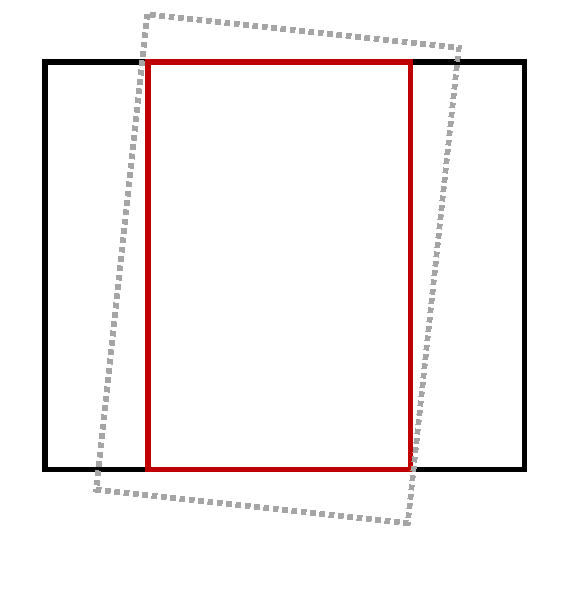
\includegraphics[width=0.9in]{projectionWallCrop.pdf}}
  \caption{(a) Images for vertical planes are tilted, but their camera
    axes are more or less normal to their respective planes. (b)
    Camera axes for ceiling images are at large angles with respect to
    plane normals. (c) Wall images are cropped to be rectangular.}
  \label{fig:projectionAngles}
\end{figure}

\subsection{Shortest Path Texturing}
\label{sec:shortestPath}

As mentioned earlier, our data comes from a mobile backpack system
carried by am ambulatory human operator, typically bent forwards at 15
to 20 degrees with respect to the vertical direction. As a result,
cameras facing sideways are head on with respect to vertical walls, as
shown in Figure \ref{fig:projectionAngles}(a), while cameras oriented
towards the top or bottom of the backpack are at an angle with respect
to horizontal floors and ceilings, as shown in Figure
\ref{fig:projectionAngles}(b). These oblique camera angles for
horizontal surfaces translate into textures that span large areas once
projected, as shown in Figure \ref{fig:projectionAngles}(b). Using the
tile-based texture mapping criteria from Figure
\ref{fig:scoringFunction}, such projections have highly varying scores
depending on the location of a tile on the plane. Thus, the tiling
approach in Section \ref{sec:mappingWithCaching} is an appropriate
choice for texturing floors and ceilings, as it uses the parts of
image projections that maximize resolution for their respective plane
locations, e.g. areas near point A and not near point B, in Figure
\ref{fig:projectionAngles}(b).


For vertical walls however, most images are taken from close distances
and head-on angles, resulting in high resolution fronto-parallel
projections. As a result, for each tile on a wall plane, the scoring
function of Figure \ref{fig:scoringFunction} is relatively flat with
respect to candidate images, as they are all more or less head
on. Since the scoring function is less discriminative for walls, it is
conceivable to devise a different texturing strategy to directly
minimize visible seams when texturing them. This is done by choosing
the smallest possible subset of images from the set selected in
Section \ref{sec:simpleTextureMapping} and aligned in Section
\ref{sec:2dAlignment} such that it (a) covers the entire plane and (b)
minimizes the visibility of borders between the images. A
straightforward cost function that accomplishes the latter is the sum
of squared differences (SSD) of pixels in overlapping regions between
all pairs of images. Minimizing this cost function encourages image
boundaries to occur either in featureless areas, such as bare walls,
or in areas where images match extremely well.

In its most general form, our problem can be defined as minimally
covering a polygon i.e. the planar surface, using other polygons of
arbitrary geometry i.e. image projections, with the added constraint
of minimizing the cost function between chosen images. Given that
wall-texture candidate images are taken from more or less head-on
angles, and knowing that only minor rotations are made in Section
\ref{sec:2dAlignment}, we can crop our image projections to be
rectangular with minimal texture loss as shown in Figure
\ref{fig:projectionAngles}(c). Furthermore, because the fisheye camera
lenses have full floor-to-ceiling coverage of nearly all walls, and
the backpack operator logically only moves horizontally, we only need
to ensure lateral coverage of our wall planes. We can thus construct a
Directed Acyclic Graph (DAG) from the images, with edge costs defined
by the SSD cost function, and solve a simple shortest path problem to
find an optimal subset of images with regard to the SSD cost function
\cite{dijkstra}.

\begin{figure}
  \centering
  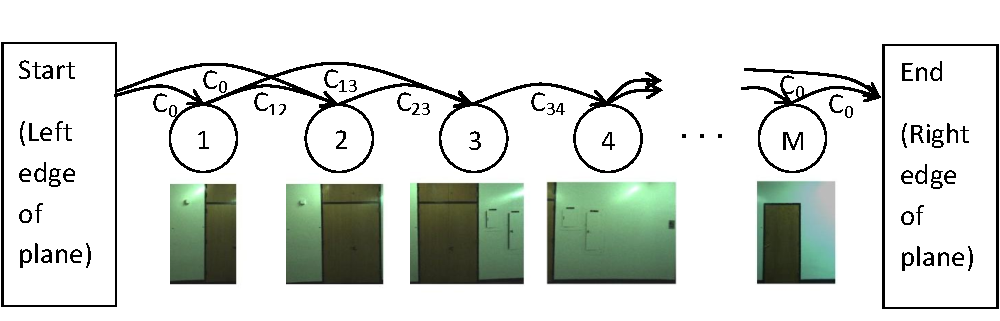
\includegraphics[width=5in]{dagCreation.pdf}
  \caption{DAG construction for the image selection process. \\}
  \label{fig:dagCreation}
\end{figure}

Figure \ref{fig:dagCreation} demonstrates the construction of a DAG
from overlapping images of a hallway wall. Images are sorted by
horizontal location left to right, and become nodes in a
graph. Directed edges are placed in the graph from left to right
between overlapping images. The weights of these edges are determined
by the SSD cost function. Next, we add two artificial nodes, one start
node representing the left border of the plane, and one end node
representing the right border of the plane. The left(right) artificial
node has directed edges with equal and arbitrary cost $C_0$ to(from)
all images that meet the left(right) border of the plane. We now solve
the shortest path problem from the start node to the end node. This
results in a set of images completely covering the plane horizontally,
while minimizing the cost of seams between images.

In rare cases where the vertical dimension of the plane is not
entirely covered by one or more chosen images, we are left with holes
where no images are selected to texture. Since these holes are rare,
and generally fairly small, we use a greedy approach, repeatedly
filling the hole with images that result in the lowest SSD costs in a
blending region around the hole, as discussed in Section
\ref{sec:blending}. This method is not optimal as a true 2D-coverage
solution would be, but it is a fast approximation, and adequately
handles the few holes encountered.

We have now (a) mapped every location on the plane to at least one
image, (b) decreased the number of texturing images, generally
retaining around 20\% of the image subset obtained in Section
\ref{sec:simpleTextureMapping}, and (c) decreased the discontinuities
at each image border. As seen in Figure \ref{fig:compareAll}(d), this
shortest path method has fewer visible discontinuities than Figure
\ref{fig:compareAll}(c) corresponding to the tile caching
approach\footnote{In Figure \ref{fig:compareAll}(d), we arbitrarily
  chose one image for texturing where images overlap, as blending will
  be discussed in section \ref{sec:blending}.}. This is especially
evident when comparing the posters in the images. This shortest path
approach directly reduces the cost of each image boundary,
while the tile caching method uses a scoring function that only
approximates this effect. Furthermore, this approach guarantees the
best selection of images to minimize seams, while the sequential tile
caching method may select images early on that turn out to be poor
choices once subsequent tiles have been processed. This shortest path
approach is also far less intensive in terms of memory usage and
runtime, both during texture generation and rendering, as it does not
require discretizing planes or images.

When texturing an entire 3D planar model, we apply the shortest path
method on walls, due to its superior results when provided with
head-on images. Floors and ceilings however, given their many images
taken at oblique angles, are textured using the tile caching method of
Section \ref{sec:mappingWithCaching}.


\subsection{Blending}
\label{sec:blending}
We now apply a blending procedure to the texturing methods in Sections
\ref{sec:mappingWithCaching} and \ref{sec:shortestPath}. Although the
image alignment steps and image selection in both methods attempt to
minimize all mismatches between images, there are occasional
unavoidable discontinuities in the final texture due to different
lighting conditions or inaccuracies in model geometry. These can
however be treated and smoothed over by applying alpha blending over
image seams.  Whether the units to be blended are
rectangularly-cropped images or rectangular tiles, we can apply the
same blending procedure, as long as there is a guaranteed overlap
between units to blend over.

For the tile caching method of Section \ref{sec:mappingWithCaching},
we can ensure overlap by texturing a larger tile than needed for
display. For example, for a rendered tile $l_1 \times l_1$, we can
associate it with a texture $(l_1 + l_2) \times (l_1 + l_2)$ in size.
We have found $l_2 = \frac{l_1}{2}$ to provide a balance between
blending and keeping features unblurred. For the shortest path method,
we have already ensured overlap between images. To enforce consistent
blending however, we add a minimum required overlap of images of 200
mm while solving the shortest path problem in Section
\ref{sec:shortestPath}. Additionally, if images overlap in a region
greater than the overlap distance, we only apply blending over an area
equal to the overlap distance.

After linear alpha blending across overlapping regions, the texture
mapping process is complete. Figures \ref{fig:compareAll}(e) and
\ref{fig:compareAll}(f) show the blended versions of Figures
\ref{fig:compareAll}(c) and \ref{fig:compareAll}(d) respectively. The
remaining images in Figure \ref{fig:compareAll} highlight differences
between the two methods, showing that Figure \ref{fig:compareAll}(f)
has the best visual quality and the best texturing approach among the
textures in Figure \ref{fig:compareAll}.

\section{Results}
\label{sec:results}
Examples of ceilings and floors textured with the tile caching
approach, and walls textured with the shortest path approach, are
displayed in Figure \ref{fig:results}. High resolution colored texture
comparisons, as well as video and interactive walkthroughs of full
models are available at
\footnote{\url{http://www-video.eecs.berkeley.edu/research/indoor/}}.

As mentioned earlier, our approach is quite efficient. The top wall in
Figure \ref{fig:results}(a) was generated with 7543 $\times$ 776
pixels, and spans a 40-meter long wall. Given 41000 input images of
the entire dataset, a 2.8GHz dual-core consumer-grade laptop takes
approximately a minute to choose 36 candidate images, followed by
under a minute to perform both image alignment and the shortest path
texturing method, though over 75\% of that time is spent calculating
SIFT matches within the SiftGPU framework, which could feasibly be
split into a separate preprocessing step. While not real-time, the
process is capable of generating fast updates after changes in various
parameters or modifications to input data, and if integrated directly
into a 3D modeling system, could provide live visualization as data is
collected. Our full models consist of an input model file, textures,
and a mapping of image points to 3D model vertices. The models shown
in Figure \ref{fig:results} are roughly 20 MB in size, and are
visualized using the OpenSceneGraph toolkit \cite{openscenegraph},
which allows for export to many common model formats, as well as
efficient visualization, even in web browsers or mobile devices.

\section{Conclusion}
\label{sec:conclusion}

In this paper, we have developed an approach to texture mapping models
with noisy camera localization data. We are able to refine image
locations based on geometry references and feature matching, and
robustly handle outliers. Using the tile-based mapping approach, we
can texture both simple rectangular walls as well as complex floor and
ceiling geometry. We also implemented a shortest path texturing method
that produces seamless textures on planes where multiple head-on
images are available. Both of these approaches are highly modular, and
easily tunable for similar systems across multiple environments.

Our method is likely to fail in scenarios where 3D error is large. A
logical progression of our approach to resolve camera error in 3D is
to perform matching between image lines and geometry in 3D, which can
be done reasonably efficiently \cite{linebased,
  rectangularstructures}. Using linear features in addition to SIFT
features is also likely to result in improved matches, as indoor
scenes often have long, unbroken lines spanning multiple images
\cite{linearposeestimation}. Finally, the blending procedure is quite
basic, and applying more sophisticated methods of blending as well as
normalization would benefit the final visual quality, and more
robustly handle motion-based or parallax errors.



\begin{figure}
  \centering
  \subfloat[][]{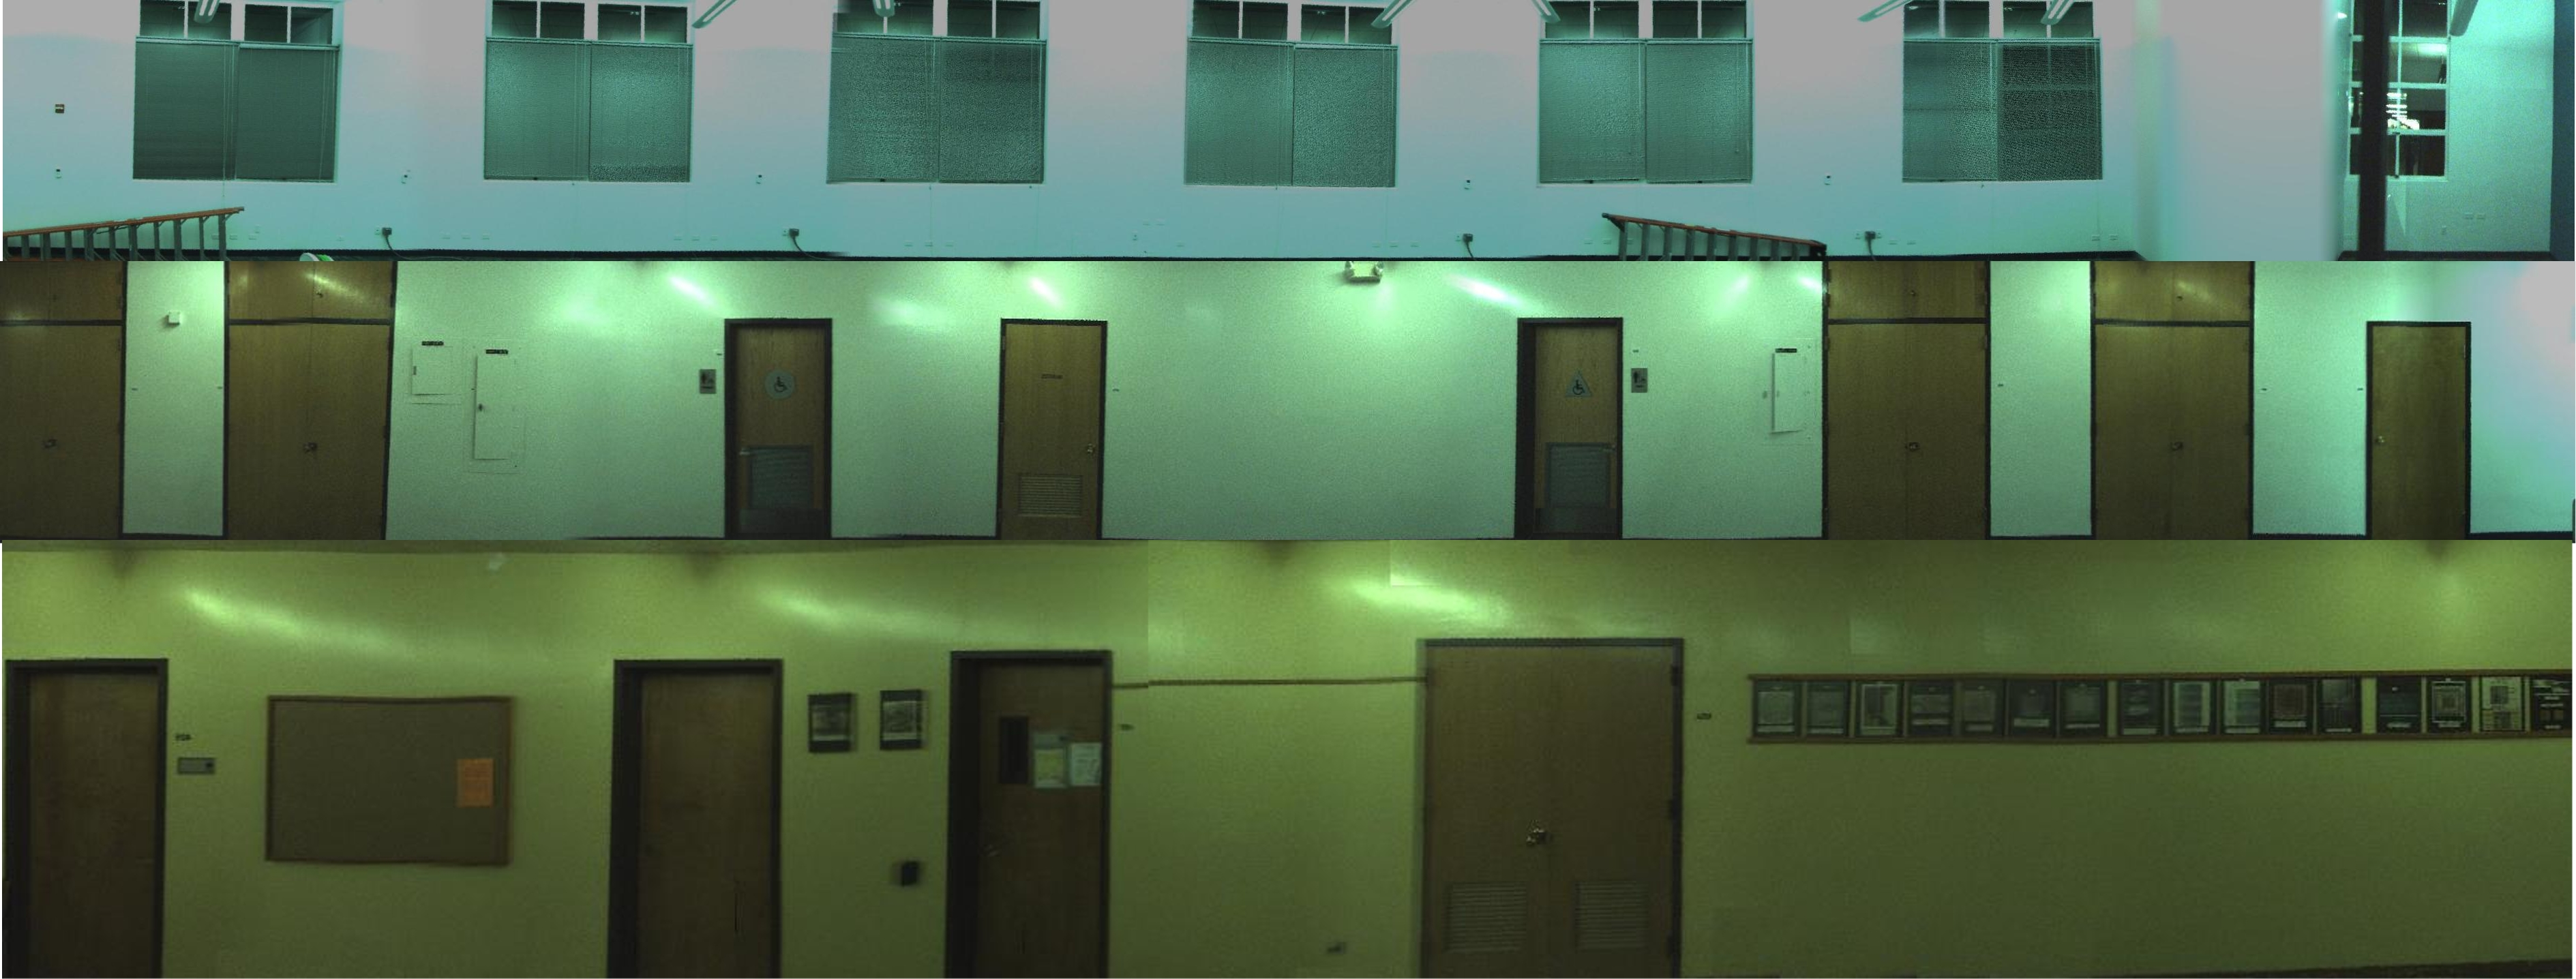
\includegraphics[width=3in]{finalfloors.jpg}} ~~~~~~~~
  \centering
  \subfloat[][]{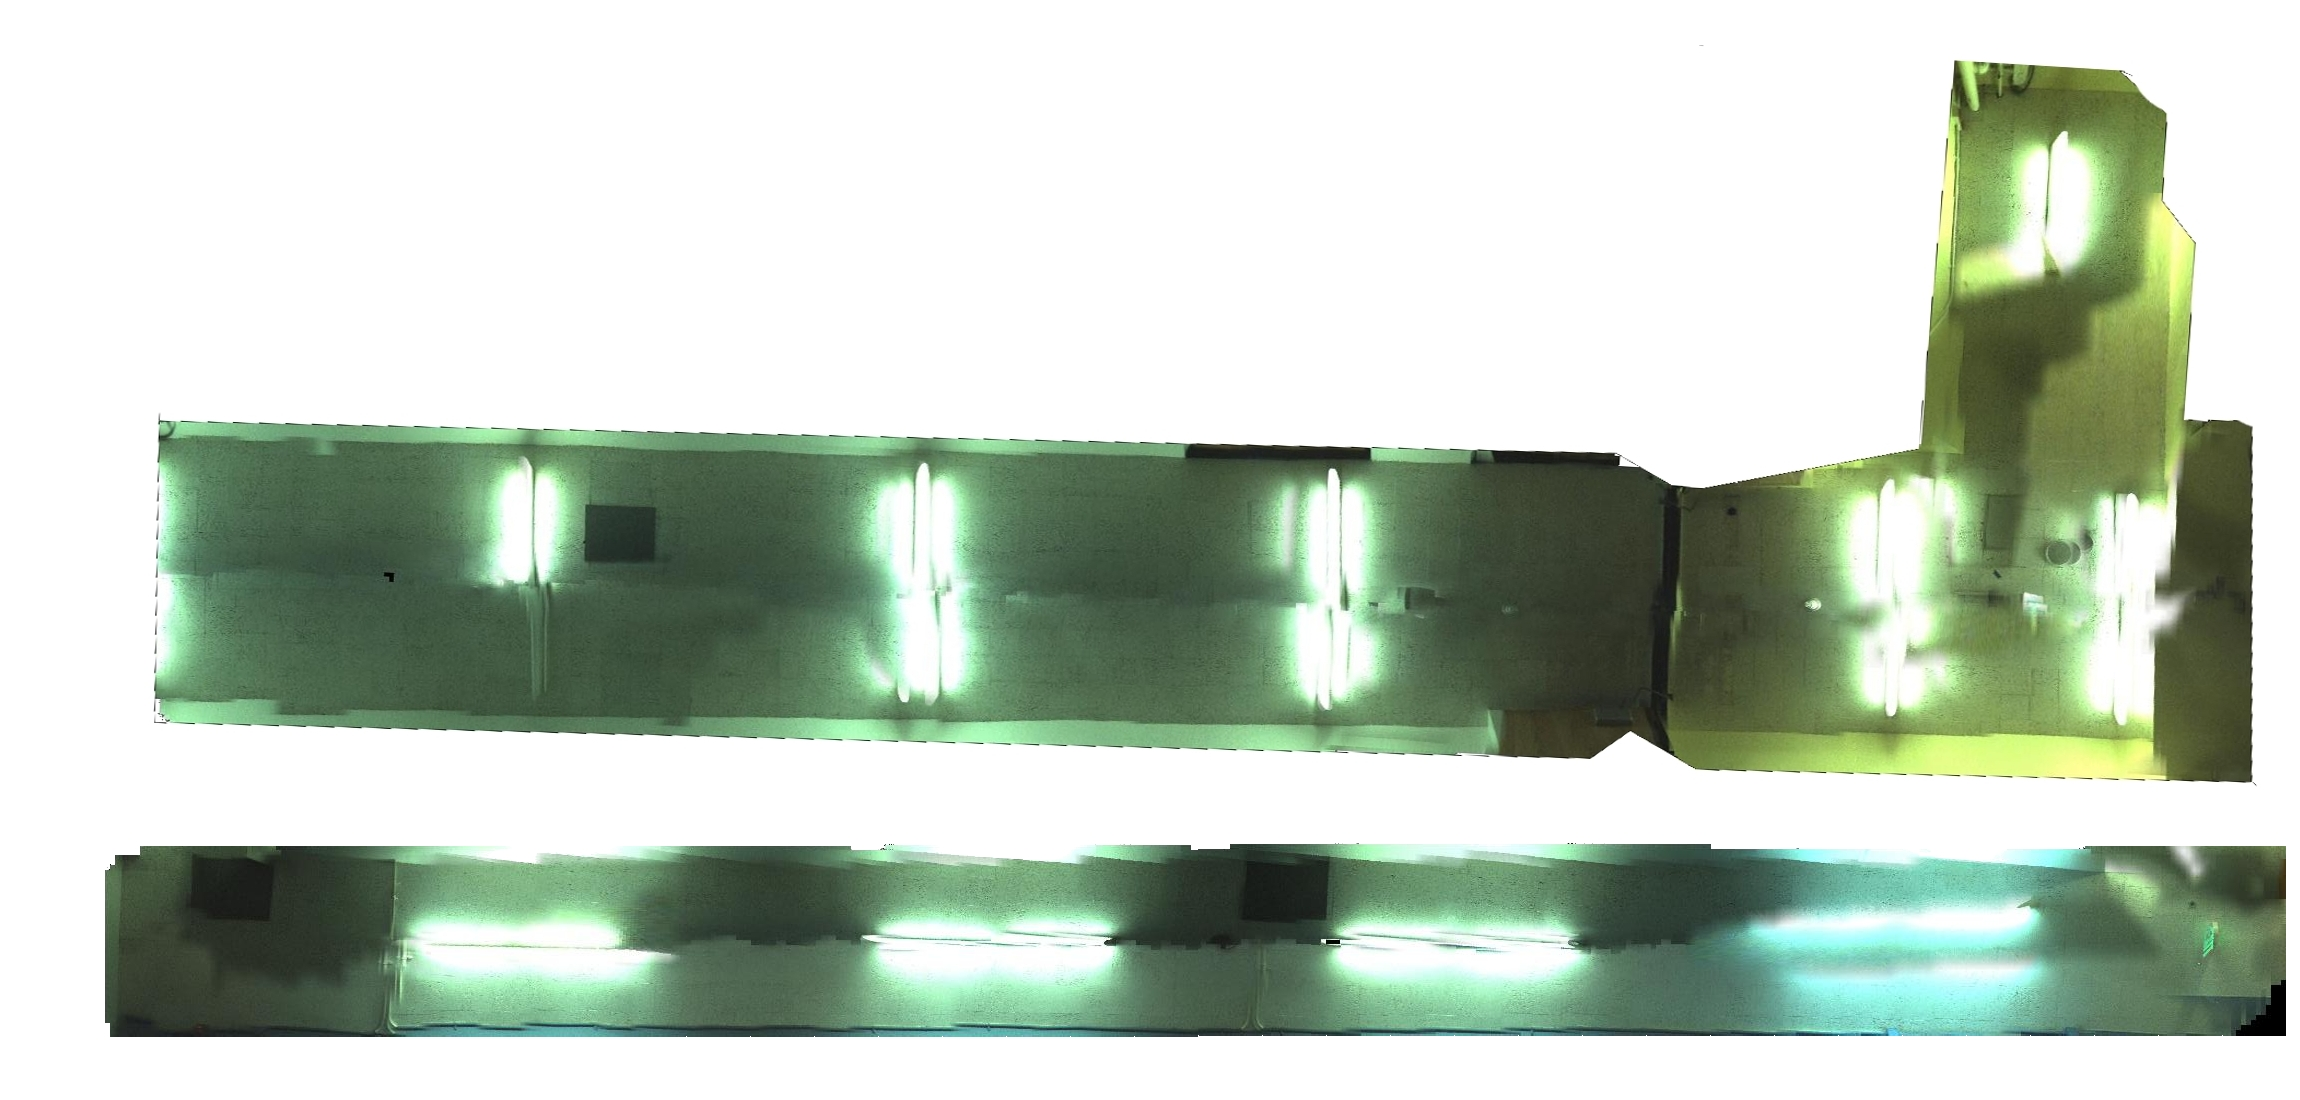
\includegraphics[width=3in]{finalceilings.jpg}}

  \centering \subfloat[][]{
    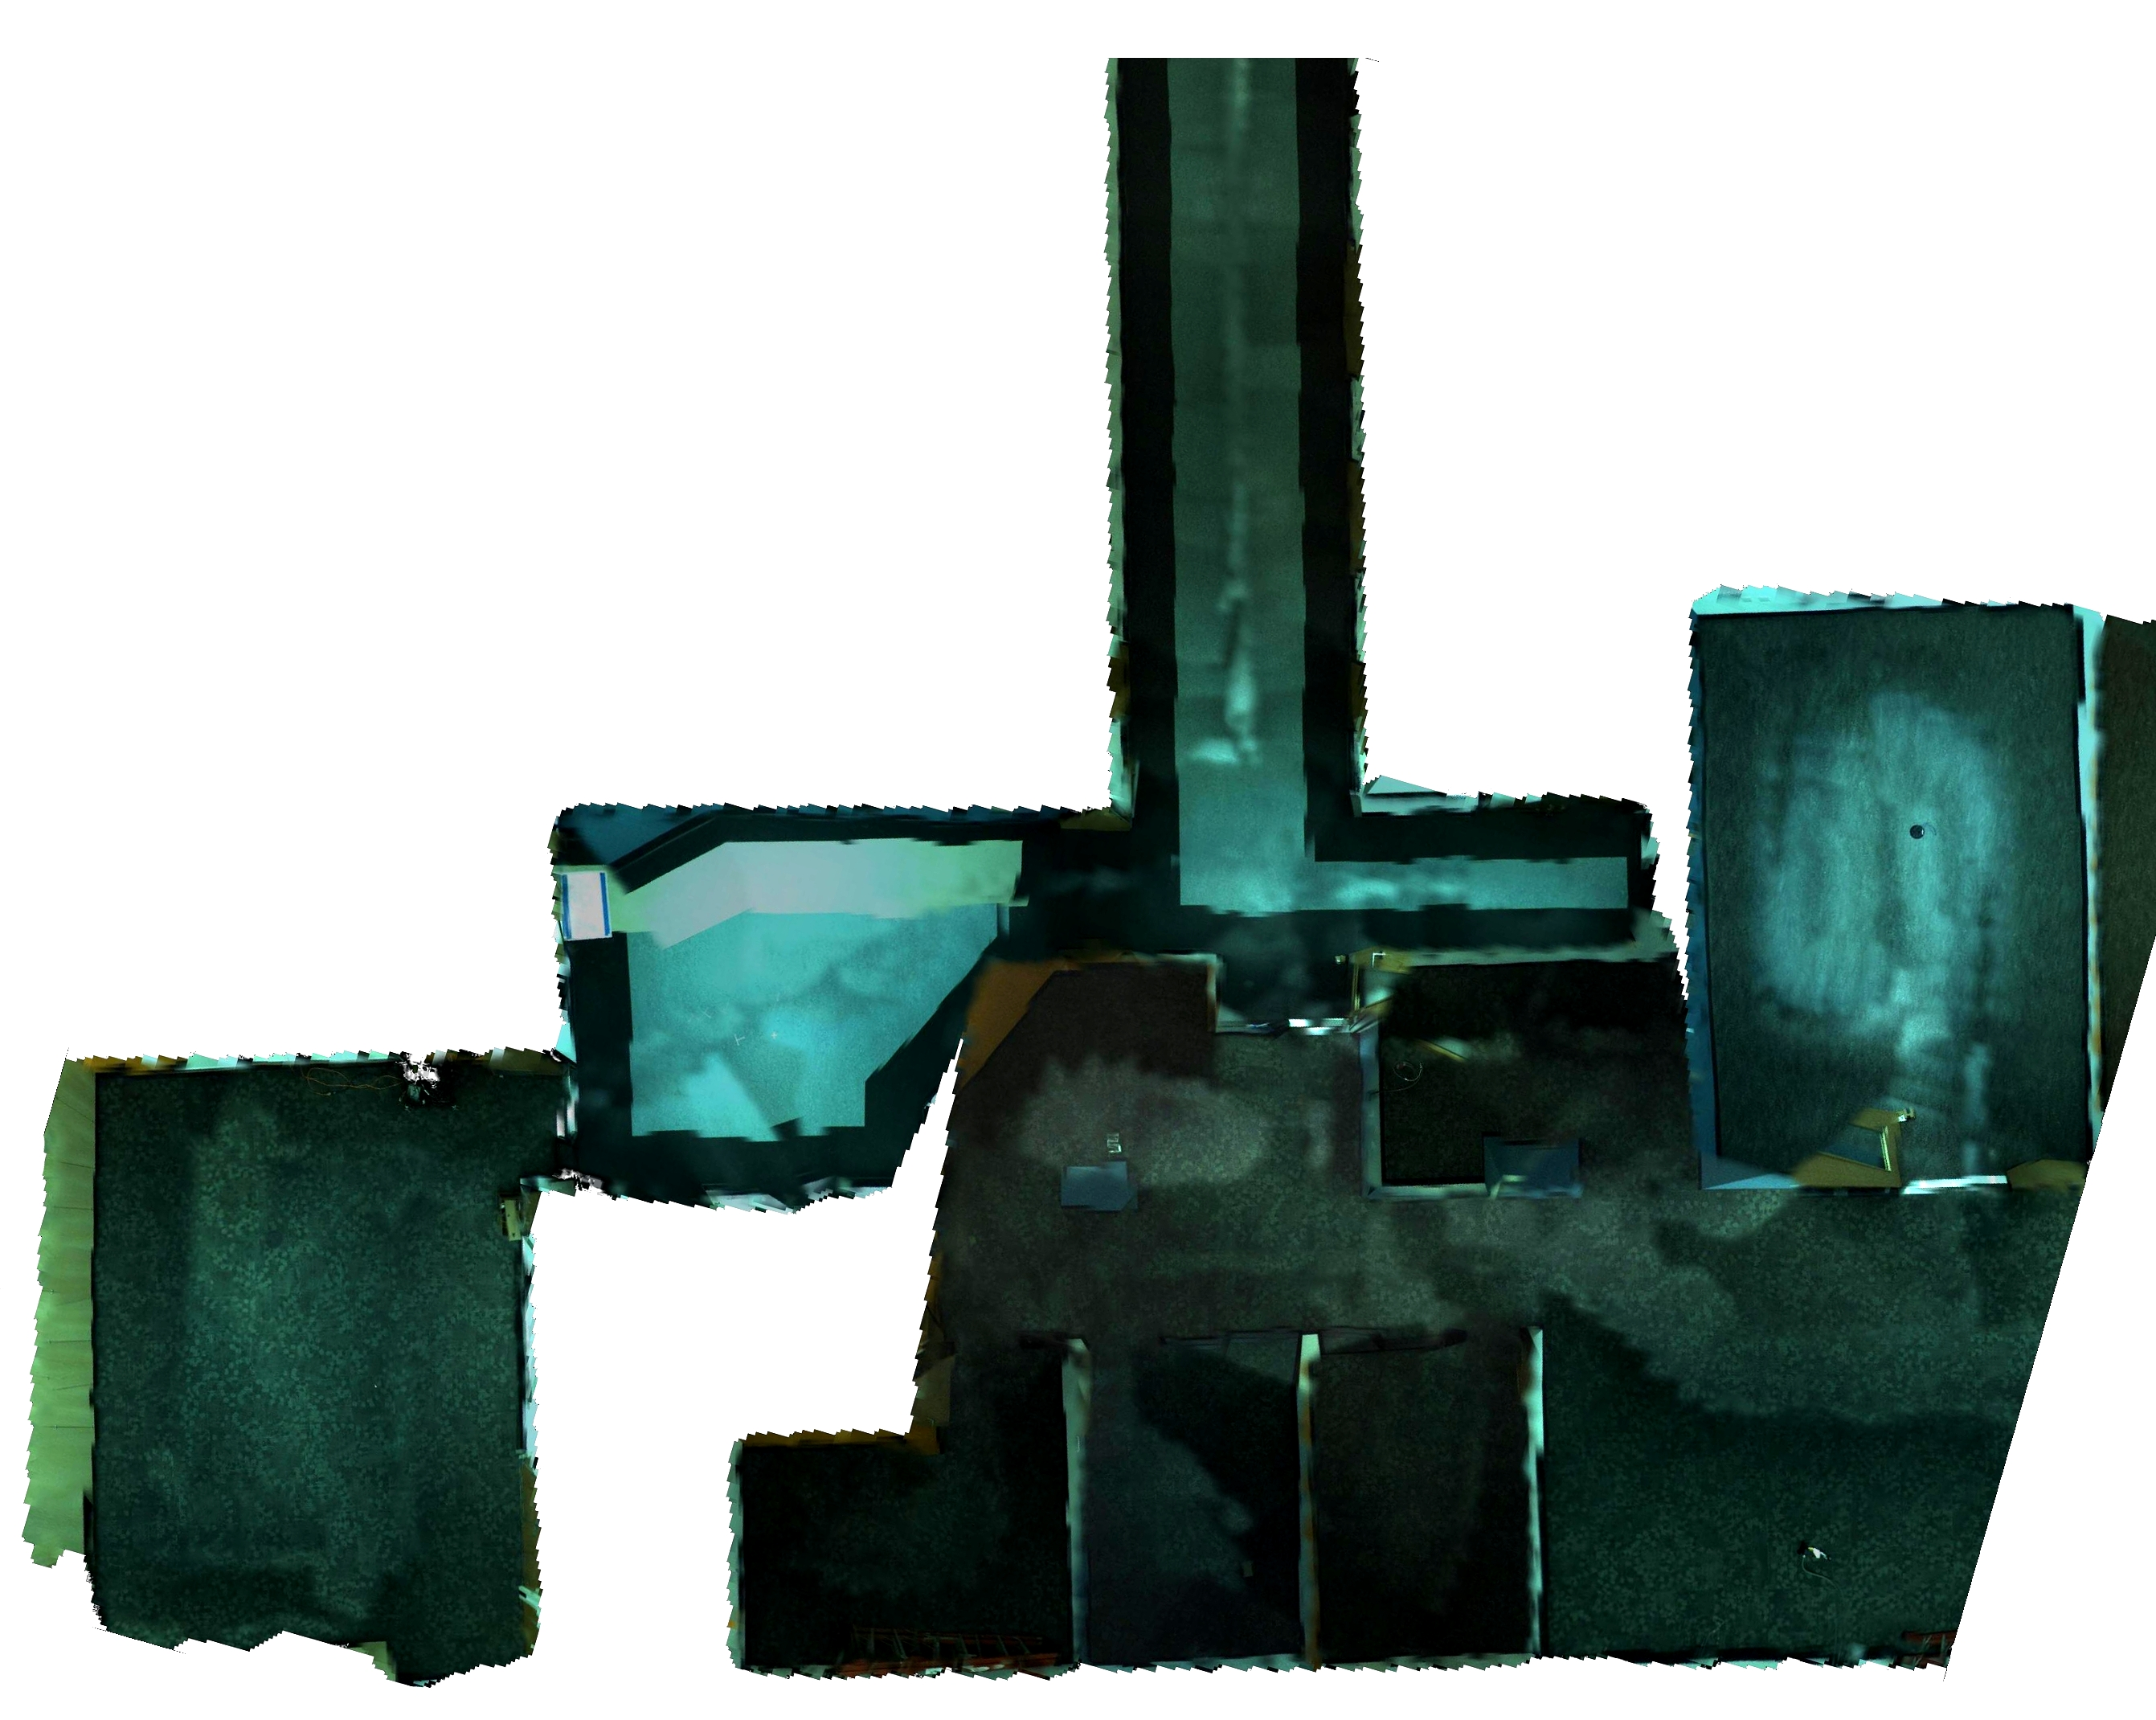
\includegraphics[height=2in, width=3in]{floorcropped.jpg} ~~~~~~~~
    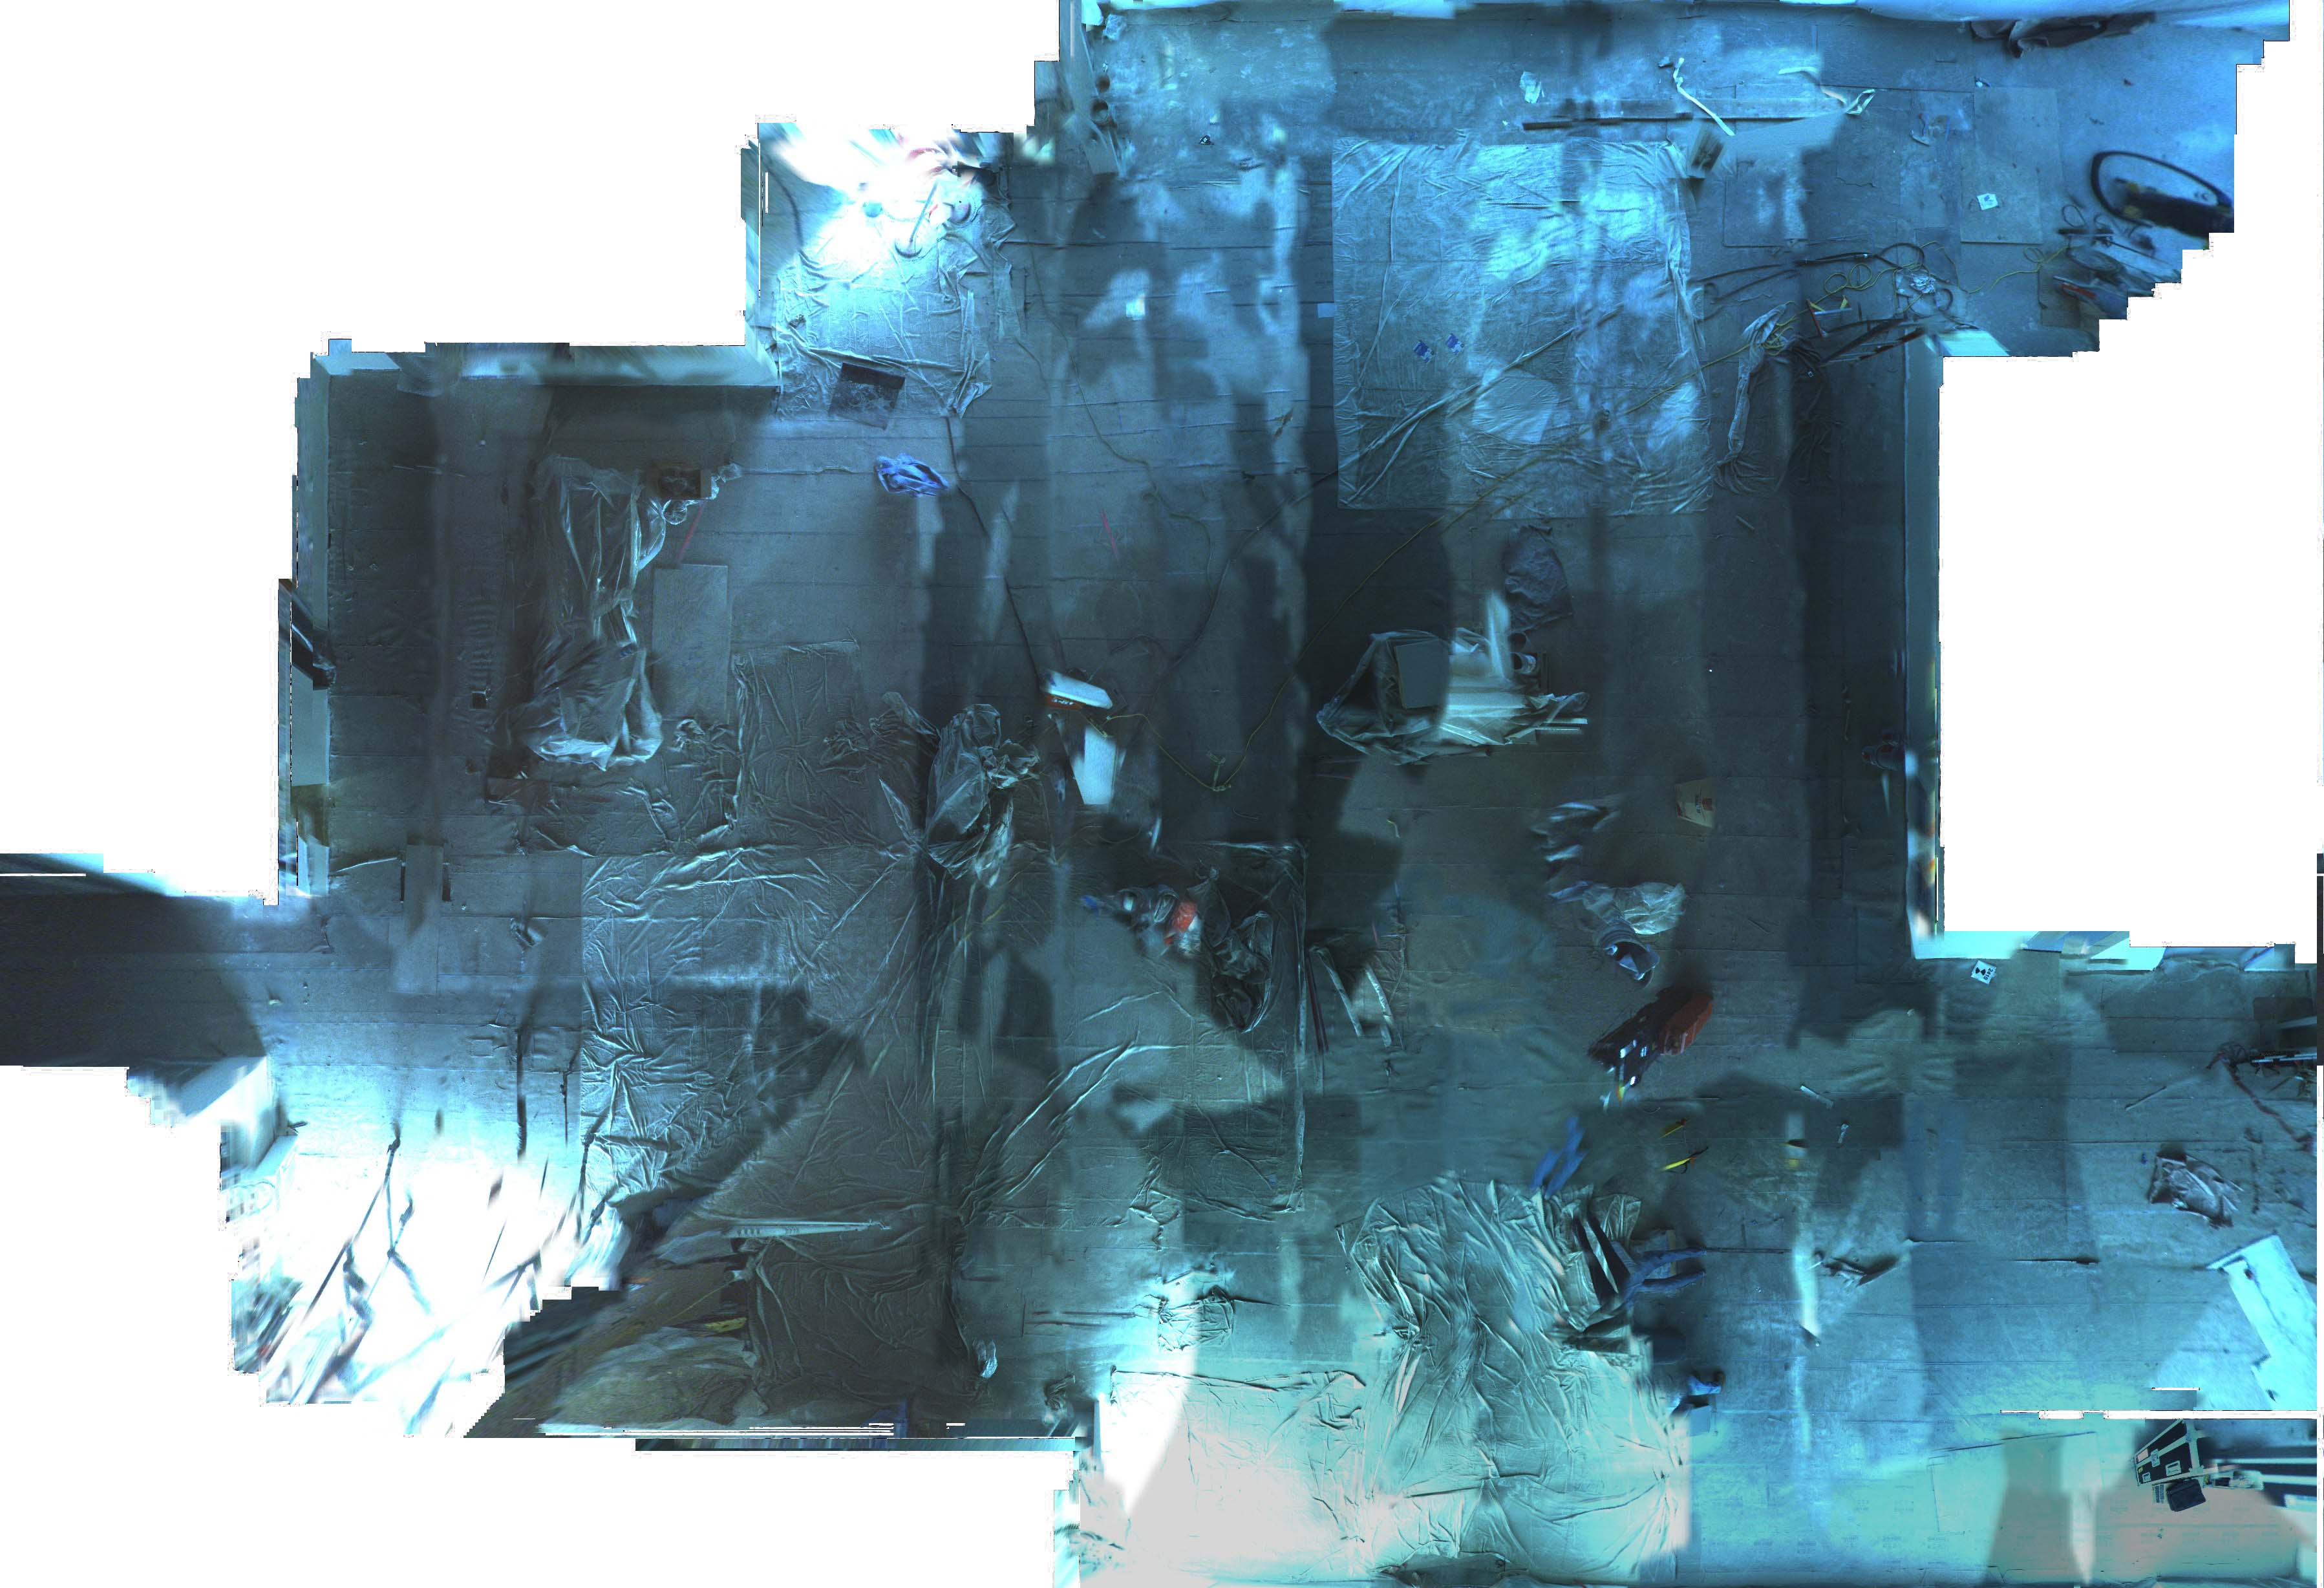
\includegraphics[width=3in]{pier15floor.jpg}
  }

  \centering{
    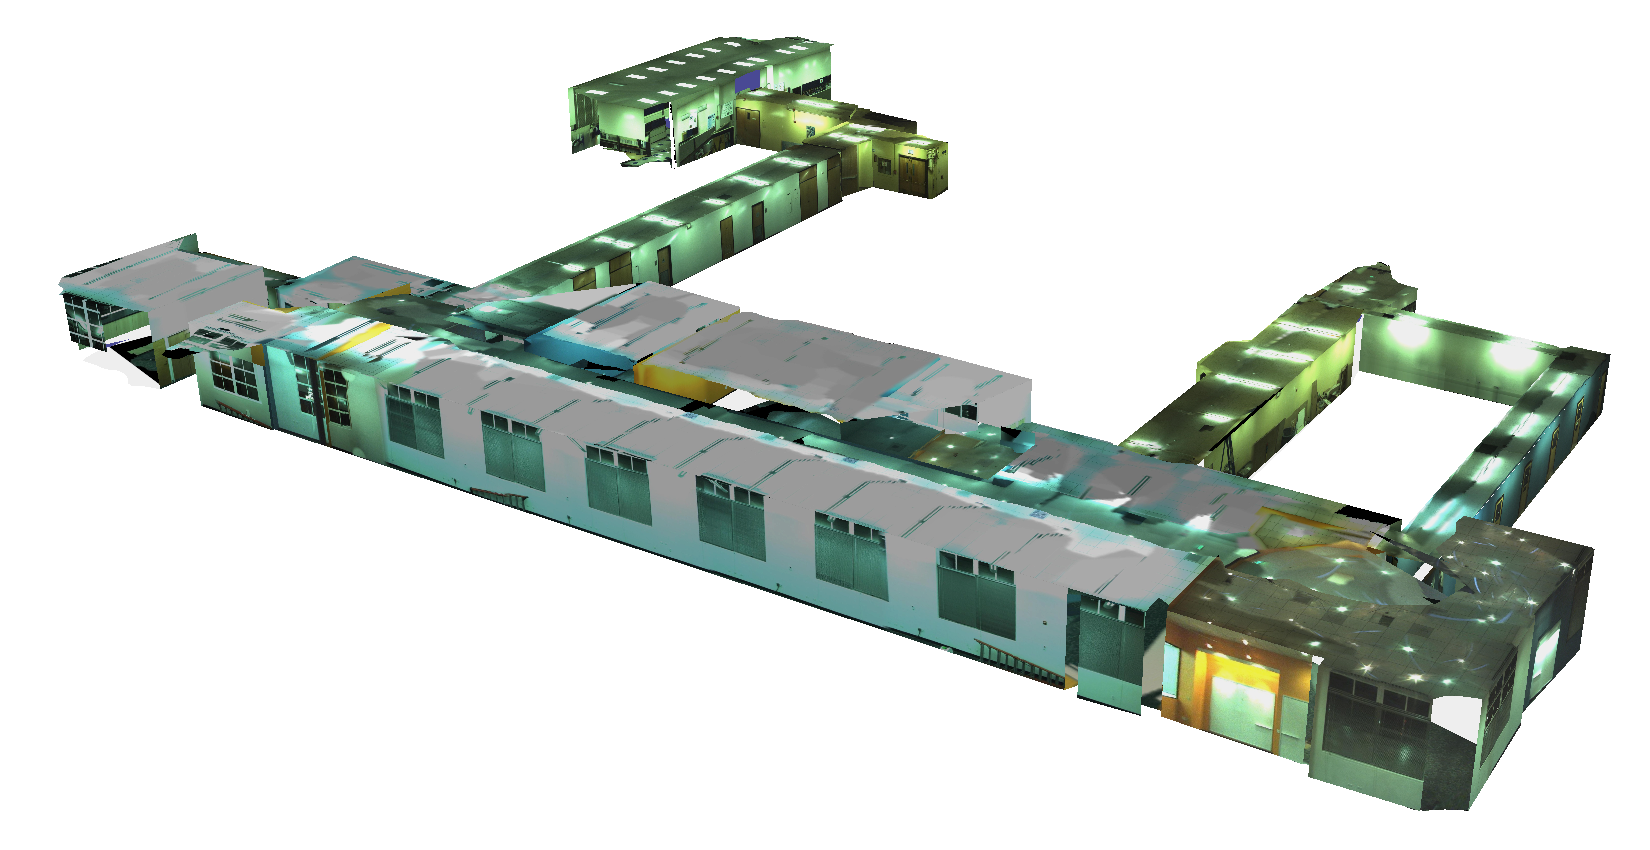
\includegraphics[width=3in]{fullmodel.png}
    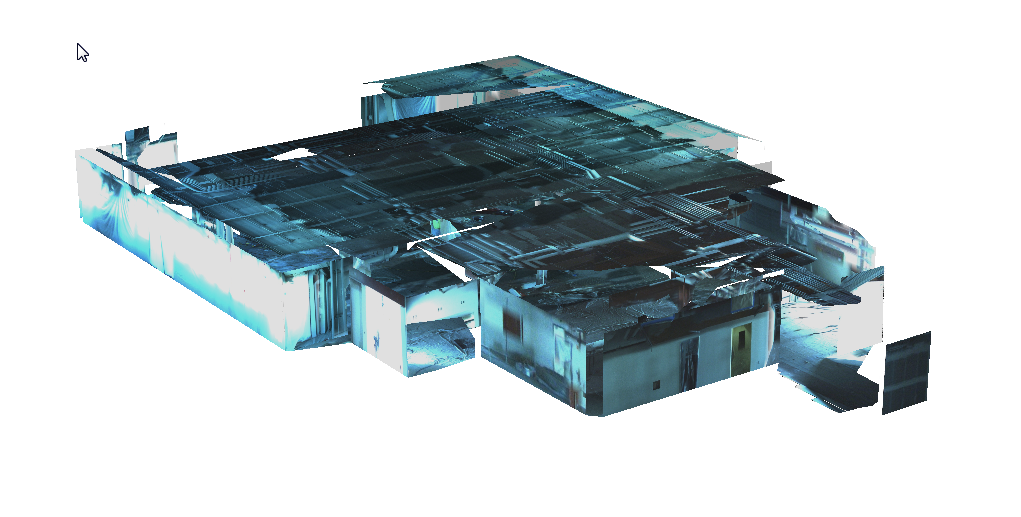
\includegraphics[width=3in]{pier15.png} \\
    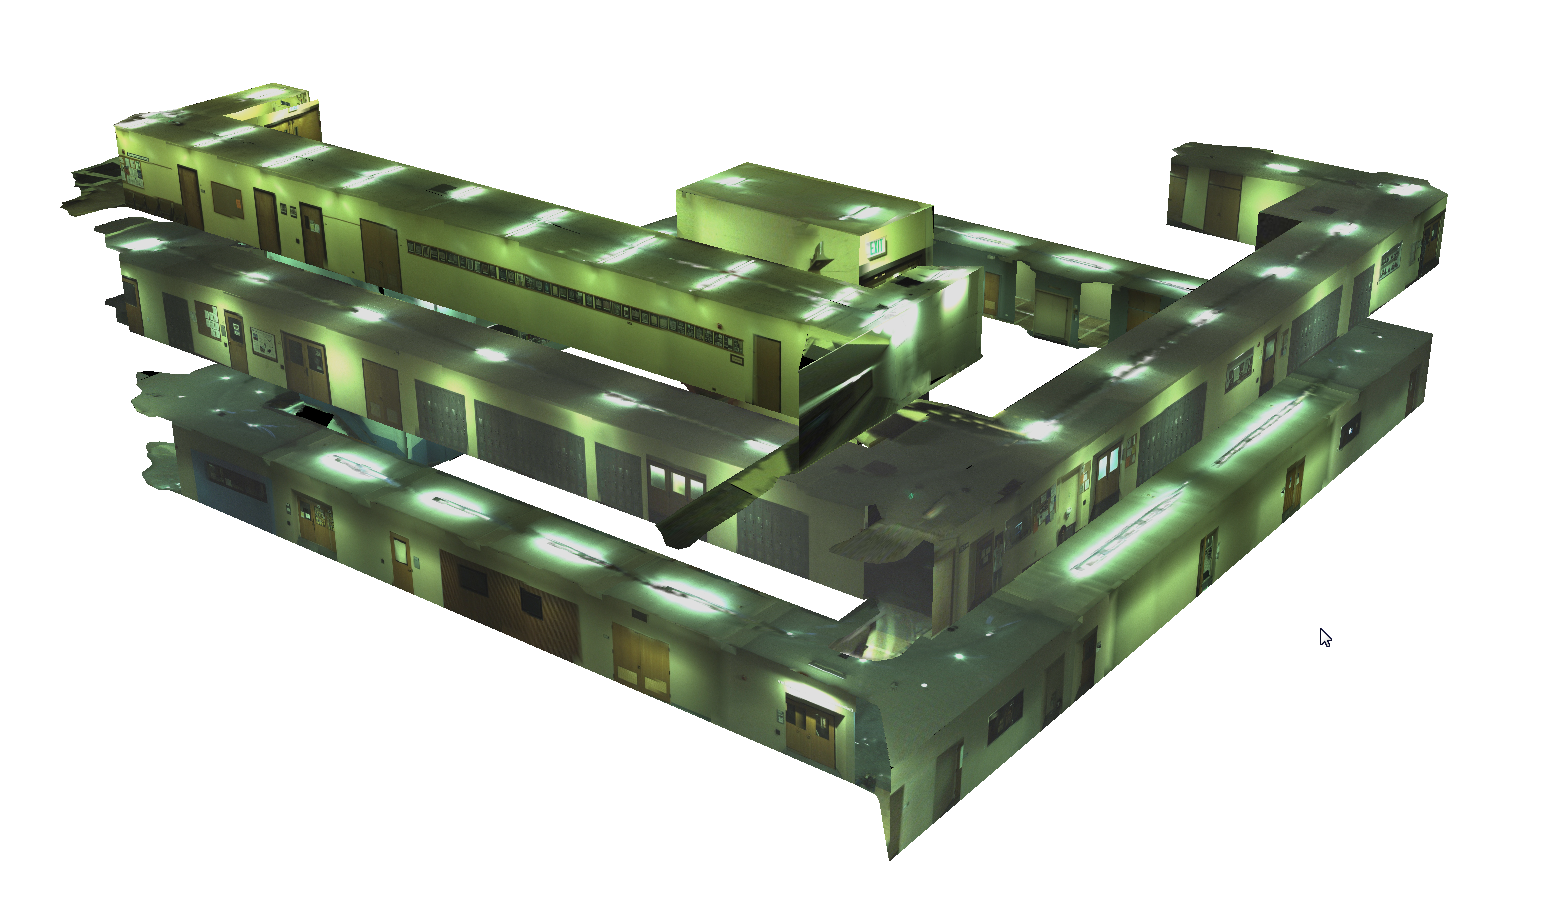
\includegraphics[width=3in]{threestoryfull2.png}
    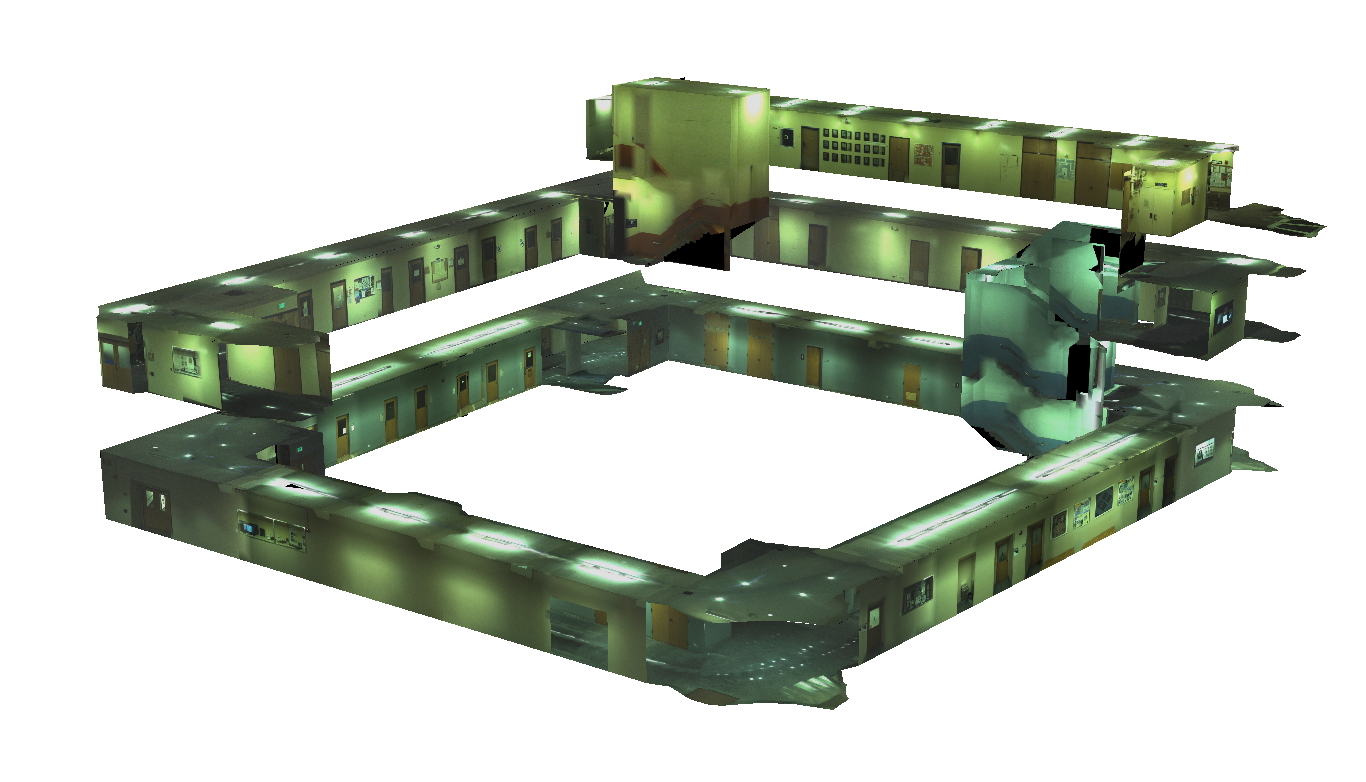
\includegraphics[width=3in]{threestoryfull.png}
  }

  \centering \subfloat[][]{ }
  \caption{Examples of our final texture mapping output for (a) walls,
    (b) ceilings, (c) floors, (d) full models.}
  \label{fig:results}
\end{figure}


%%%%%%%%%%%%%%%%%%%%%%%%%%%%%%%%%%%%%%%%%%%%%%%%%%%%%%%%%%%%%
%%%%% References %%%%%

\bibliography{report} %>>>> bibliography data in report.bib
\bibliographystyle{spiebib} %>>>> makes bibtex use spiebib.bst

\end{document} 
